\documentclass[a4paper,10pt]{article}

\usepackage{fullpage}
\usepackage{graphicx}
\usepackage{amsmath}
\usepackage{amssymb}
\usepackage{hyperref}
\hypersetup{
    colorlinks=true,       % false: boxed links; true: colored links
    linkcolor=blue,          % color of internal links
    citecolor=green,        % color of links to bibliography
    filecolor=magenta,      % color of file links
    urlcolor=cyan           % color of external links
}

\usepackage{epsfig}


% Title Page
\title{Baby Brain Toolkit}
\author{Fbrain ERC project: Computational Anatomy of Fetal Brain}


\begin{document}
\maketitle
\tableofcontents
%\begin{abstract}
%\end{abstract}

\section{Introduction}

BTK stands for Baby Brain Toolkit. This toolkit is developed in the context of
the Fbrain ERC project: ``Computational Anatomy of Fetal
Brain''\footnote{http://lsiit-miv.u-strasbg.fr/miv/index.php?contenu=erc}. 
Studies about brain maturation aim at providing a better understanding of brain
development and links between brain changes and cognitive development. Such
studies are of great interest for diagnosis help and clinical course of
development and treatment of illnesses. Several teams have begun to make 3D maps
of developing brain structures from children to young adults. However, working
out the development of fetal and neonatal brain remains an open issue. This
project aims at jumping over several theoretical and practical barriers and at
going beyond the formal description of the brain maturation thanks to the
development of a realistic numerical model of brain aging.

\subsection{Copyright}
This software is governed by the CeCILL-B license under French law and
abiding by the rules of distribution of free software.  You can  use, 
modify and/ or redistribute the software under the terms of the CeCILL-B
license as circulated by CEA, CNRS and INRIA at the following URL: \url{http://www.cecill.info}. 

As a counterpart to the access to the source code and rights to copy,
modify and redistribute granted by the license, users are provided only
with a limited warranty  and the software's author,  the holder of the
economic rights,  and the successive licensors  have only  limited
liability. 

In this respect, the user's attention is drawn to the risks associated
with loading,  using,  modifying and/or developing or reproducing the
software by the user in light of its specific status of free software,
that may mean  that it is complicated to manipulate,  and  that  also
therefore means  that it is reserved for developers  and  experienced
professionals having in-depth computer knowledge. Users are therefore
encouraged to load and test the software's suitability as regards their
requirements in conditions enabling the security of their systems and/or 
data to be ensured and,  more generally, to use and operate it in the 
same conditions as regards security. 

Any researcher reporting results using BTK should acknowledge this software by citing the following article:
\begin{enumerate}
\item F. Rousseau, E. Oubel, J. Pontabry, C. Studholme, M. Koob, J.-L. Dietemann: BTK: An Open-Source Toolkit for Fetal Brain MR Image Processing. Research Report, October 2011, available on \href{http://hal.archives-ouvertes.fr/index.php?halsid=d0mrvug09qhhou49vgaqc6ogd3&view_this_doc=hal-00671183&version=1}{HAL}.
\end{enumerate}

\subsection{Installation}

\subsubsection{Dependencies}

Baby Brain Toolkit (BTK) needs the following packages\footnote{BTK has been tested under Debian 5.0 and MacOSX 10.6.8}:
\begin{itemize}
 \item \href{http://www.cmake.org}{CMake}, \href{http://tclap.sourceforge.net}{Tclap}, \href{http://openmp.org}{OpenMP}, \href{http://www.vtk.org}{VTK}, ANN (www.cs.umd.edu/\string~mount/ANN) and Doxygen. These
libraries can be installed using the following command line: 
 \begin{itemize}
 \item for debian-based distributions: \texttt{apt-get install cmake
cmake-curses-gui libtclap-dev libgomp1 libvtk5-dev libann-dev doxygen}
 \item for MacOSX using macports\footnote{When configuring in cmake, please use /opt/local/include for TCLAP\_DIRECTORY}: \texttt{port install cmake tclap vtk5 libANN doxygen}
 \end{itemize}
 \item Install Git: this library can be installed using the following command line : 
 \begin{itemize}
 \item for debian-based distribution: \texttt{apt-get install git-core}
 \item for MacOSX using macports: \texttt{port install git-core}
 \end{itemize}
 \item \href{http://www.itk.org/ITK/resources/software.html}{Insight Toolkit (ITK) version 4}
 \begin{itemize}
 \item Download the tar.gz archive of ITK v4.0
 \item Extract the archive 
 \item Then open a terminal and type :
 \end{itemize}
\begin{verbatim}
mkdir ITK-build
cd ITK-build
ccmake ../(your-ITK-Source-folder)/
\end{verbatim}
This will bring up the CMake configuration screen. Press \texttt{[c]} for
configure and then use \texttt{[t]} to toggle the advanced mode. Make the
following changes:
\begin{verbatim}
BUILD_TESTING = OFF
CMAKE_BUILD_TYPE = Release
ITK_USE_REVIEW = ON
ITK_BUILD_ALL_MODULES = ON
ITKV3_COMPATIBILITY = ON
BUILD_DOCUMENTATION = OFF
\end{verbatim}
Then press \texttt{[c]} to configure and \texttt{[g]} to generate the make file.
Finally, go to the build folder of ITK (ITK-build) and type \texttt{make} at the prompt to obtain the final build of ITK.

\end{itemize}

\subsubsection{Download and compile the BTK sources}
\begin{itemize}
 \item Get the BTK sources: \texttt{git clone https://github.com/rousseau/fbrain.git }
 \item Then:
\begin{verbatim}
mkdir fbrain-build
cd fbrain-build
ccmake ../fbrain
make
\end{verbatim}
\end{itemize}

Most of the programs of the BTK suite use the OpenMP library for multi-threading
purpose\footnote{Please note that the current Apple compiler (llvm gcc 4.2.1) does not take into account OpenMP.}. The number of cores used can be tuned using the following command line
(in this example, 4 cores will be used): \texttt{export OMP\_NUM\_THREADS=4}
\section{The BTK pipeline}
BTK allows to implement a pipeline for the processing of fetal images,
i.e. the reconstruction of anatomical and diffusion data, and the final
tractography, all expressed in the same local coordinate system. This
processing can be summarized in the following steps: 1) image conversion, 2) anatomical image reconstruction, 3)
recontruction of the diffusion sequence, 4) registration of diffusion to anatomical data and 5)
tractography.

\subsection{Image conversion}
BTK supports and has been tested by using images in Nifti format
(http://nifti.nimh.nih.gov/nifti-1). However, images are frequently available in
DICOM format and an image conversion is required. This can be performed by using
dcm2nii (http://www.cabiatl.com/mricro/mricron/dcm2nii.html), Slicer or other softwares.

Let say that you have 3 (possibly orthogonal) anatomical images:
\begin{verbatim}
ana01.nii.gz 
ana02.nii.gz 
ana03.nii.gz 
\end{verbatim}

and one set of DWI images: 
\begin{verbatim}
dwi.nii.gz
dwi.bvec 
dwi.bval 
\end{verbatim}

Please check that images are not flipped.\\

\underline{NOTE}: The set of three files .nii.gz, .bvec, and .bval used to
describe a DW sequences are represented in BTK just by the basename (``dwi'' in
the previous example), and the sequences must be provided in this way to the
different applications. This allows to have shorter command lines and a the use
of consistent filenames.

\subsection{Anatomical image reconstruction}
Anatomical image reconstruction can be performed by using \textbf{btkImageReconstruction} (Section
\ref{subsec:ana_rec})\footnote{Best results are obtained by using a mask for each anatomical image. Such image masks can be easily created using ITKSnap for instance.}, followed by a re-orientation procedure using \textbf{btkSetStandardCoorSystem} and \textbf{btkReorientImageToStandard} (Section \ref{sec:utilities})\footnote{Note that the landmarks file is obtained using external software (Slicer). Please see Section \ref{sec:utilities} for details about this step.}:

\begin{verbatim}
 
btkImageReconstruction -i ana01.nii.gz -i ana02.nii.gz -i ana03.nii.gz 
                       -m ana01_mask.nii.gz -m ana02_mask.nii.gz -m ana03_mask.nii.gz
                       -o ana3D.nii.gz --mask

btkSetStandardCoorSystem -i ana3D.nii.gz -o ana3D_standard.nii.gz -d 3
btkReorientImageToStandard -i ana3D_standard.nii.gz -o ana3D_oriented.nii.gz -l landmarks.fcsv

\end{verbatim}



\subsection{Reconstruction of the diffusion sequence}
To reconstruct diffusion data, you want to follow the steps described in
Section \ref{subsec:diff_rec}. The use of two applications is required here:
\textbf{btkGroupwiseS2SDistortionCorrection} and
\textbf{btkRBFInterpolationS2S}.

\subsection{Registration of diffusion to anatomical data}
This can be performed by using \textbf{btkRegisterDiffusionToAnatomicalData}
(Section \ref{subsec:ana_rec})

\subsection{Tractography}
If you have followed the previous steps correctly, at this point you should
have the reconstructed anatomical and diffusion data spatially aligned, and
ready to perform the tractography. To do this, BTK provides
\textbf{btkTractography} (Section \ref{subsec:tracto}).

\section{Applications}

\subsection{Denoising \cite{coupe_2008}}

\begin{description}
 \item[btkNLMDenoising] This program applies a non-local mean filter to a 3D
image  for denoising purpose. Usage: \texttt{-i input\_image\_filename -o
output\_image\_filename}. The best results are usually obtained by using a mask
(or a padding value). This is an implementation of the method proposed by Coup\'e \textit{et al.} in \cite{coupe_2008}.
\end{description}

\begin{description}
 \item[btkNLMDenoising4DImage] This program applies a non-local mean filter to 
 each 3D image of a 4D image, for denoising purpose. Usage: \texttt{-i
input\_image\_filename -o output\_image\_filename}. The best results are usually
obtained by using a mask (or a padding value).
\end{description}


\subsection{Anatomical reconstruction}
\label{subsec:ana_rec}

\begin{description}
 \item[btkImageReconstruction] This program allows to obtain a
high-resolution image from a set of low-resolution images, typically
axial, coronal, and sagittal acquisitions~(similar to \cite{rousseau_registration_2006}). \\\\
Minimal usage: \texttt{btkImageReconstruction -i image1 $\cdots$ -i imageN -o
output --box}. 

Recommended usage: \texttt{btkImageReconstruction -i image1 $\cdots$ -i imageN
-m mask1 $\cdots$ -m maskN -o output --mask}. The use of a mask provide
better results since it allows an accuratelly estimation of the initial
transform, and constrains the registration to the region of interest.

The full list of optional parameters of the method can be obtained by
\texttt{btkImageReconstruction --help}

\end{description}

\begin{description}
 \item[btkSuperResolution] To be documented. 

\end{description}

\subsection{Anatomical segmentation}
\label{subsec:ana_seg}

\begin{description}
 \item[btkTissueSegmentation] This program allows to obtain :
        \begin{itemize}
         \item A segmentation of the brain which separate pericerebral LCR and ventricules,
         \item A segmentation of the cortex inside of a region of interest defined from the border between brain and pericerebral LCR,
        \end{itemize}
        as described in~\cite{caldairou_segmentation_2011}.
        
        Usage: \texttt{btkTissueSegmentation -i greyImage -s intracranianVolume -l brainstemSegmentation -l cerebellumSegmentation -o brainSegmentation -o cortexSegmentation}
\end{description}

\begin{description}
 \item[btkLabelPropagation] This program applies a patch-based label propagation algorithm for segmentation~\cite{rousseau_supervised_2011}. As a supervised method, it takes as input a textbook containing several anatomical images and the corresponding segmentation maps.
\end{description}


\subsection{Reconstruction of DW sequences \cite{oubel_reconstruction_2010}}
\label{subsec:diff_rec}
The reconstruction of diffusion-weighted (DW) sequences aims at
obtaining a sequence corrected for fetal moving and eddy-current distortions.
This can be performed in BTK by using the two following applications. 
\begin{description}
\item[btkGroupwiseS2SDistortionCorrection] It performs a groupwise
slice-by-slice registration of the image components of the sequence.

Minimal usage: \texttt{btkGroupwiseS2SDistortionCorrection -i input -o
output -t transform-folder}.

\begin{itemize}
 \item[-i] input sequence.
 \item[-o] output sequence.
 \item[-t] folder to save the transformation files
\end{itemize}

The slice-by-slice transform for a given DW image is saved as a set of $N$
transforms in ITK format, with $N$ the number of slices in the image.

NOTE: For slice registration, 20\% of the samples are used for computing the
image metric. As the region of interest of the slice can be small, this number
of samples might be insufficient to compute the metric accurately. However,
this percent of samples has been sufficient for the tested sequences. 

\item[btkRBFInterpolationS2S] It performs an interpolation of scattered data
generated from the application of slice-by-slice transforms. To this end,
radial basis functions are used. By default, the output has isotropic
voxels of size equal to the in-plane resolution of the input.

Minimal usage: \texttt{btkRBFInterpolationS2S -i input -m mask.nii -o output
-t transformation-folder}.

\begin{itemize}
 \item[-i] input sequence
 \item[-m] mask for the B0 image
 \item[-o] output sequence 
 \item[-t] folder with the transformations generated by
\texttt{btkGroupwiseS2SDistortionCorrection}
\end{itemize}

\end{description}


\subsection{Tractography \cite{pontabry_probabilistic_2011}}
\label{subsec:tracto}

** TO BE MODIFIED ** : THIS SECTION CORRESPONDS TO THE FOLLOWING PROGRAMS: btkODFParticleFilterTractography, btkODFStreamlineTractography, btkTensorParticleFilterTractography, btkTensorStreamlineTractography, btkTractography.

    \subsubsection*{Standard usage}
        Suppose you want to perform a tractography on a diffusion weighted MRI 
dataset. You should have a dwi image, the corresponding gradient vectors'
coordinates, a mask of the brain white matter and a label image of the seeds.
Assume this data is stored in files named repsectively for instance
\texttt{data.nii.gz}, \texttt{data.bvec}, \texttt{mask.nii.gz} and
\texttt{seeds.nii.gz}. The tractography is accomplished by the command below.
            \begin{quote}
                \texttt{btkTractography -d data.nii.gz -m mask.nii.gz -l seeds.nii.gz}
            \end{quote}
        When the program terminates its task, the probability connection map and
        the fibers estimation are saved in files respectively named
\texttt{map.nii.gz} and \texttt{fibers.vtk}. The connection map is a volume
image of probability intensities (\texttt{i.e.} intensities between 0 and 1)
with the same origin, orientation and spacing as the diffusion weighted image.
The fibers are polygonal data of VTK library in world coordinates. The standard
pipeline of the program is shown in
Fig.~\ref{btkTractography-fig:standard-pipeline}.
            \begin{figure}
                \centering
                \includegraphics[width=0.6\textwidth]{btkTractographyPipeline}
                \caption{Standard pipeline of the btkTractography program.}
                \label{btkTractography-fig:standard-pipeline}
            \end{figure}

        The file named \texttt{seeds.nii.gz} is a label map which is used to 
        generate seeds for the algorithm. The spacing in millimeters between
seeds can be adjust with the option \texttt{-\hspace{0.1mm}-seed\_spacing}.

        By default, Right-Anterior-Superior (RAS) coordinate system is used to 
        ensure compatibility with Slicer3D. However, it can be forced to use
Left-Posterior-Superior (LPS) coordinate system by using option \texttt{--lps}
on command line.

        If the DWI sequence contains more than one baseline image, the program 
        takes the average of all baseline images. The baseline images can be
everywhere in the sequence. It should be recognized by null vector in
corresponding gradient's table.

    \subsubsection*{Advanced usage}
        In addition to standard arguments of \texttt{btkTractography} program, 
        there are some other parameters that let you to alter algorithm's
behaviour. These options can be classified into three groups : model's options,
constraints on trajectory and filter's options. The first group options allow
you to tweak the model (for more details about it, please refer
to~\cite{descoteaux_regularized_2007}). The second group options let you to
control the particle's trajectory. These options provide prior informations to
the algorithm. The last group options are dedicated to the particle filter
control.

        Since the default parameters values may work in the most of cases, they 
        are optional. A list is of optional features is avaible by using the
command
            \begin{quote}
                \texttt{btkTractography -\hspace{0.1mm}-help} \hspace{0.5mm} or 
                \hspace{0.5mm} \texttt{btkTractography -h}
            \end{quote}
        and program's arguments are much more described below.


    \subsubsection*{Model's order}
        The model's order (i.e. the spherical harmonics' order) can be specified
        by the option
            \begin{quote}
                \texttt{-\hspace{0.1mm}-model\_order <order>} \enspace ,
            \end{quote}
        for \texttt{order}$\;\in\{2,4,6,8\}$. The default value is 4. For more 
        details, please refer to~\cite{descoteaux_regularized_2007}.

    \subsubsection*{Model's regularization}
        A Laplace-Beltrami regularization coefficient is used to assume a better
        estimation of the model. This coefficient can by manually modified by
the option
            \begin{quote}
                \texttt{-\hspace{0.1mm}-model\_regularization <coefficient>} \enspace ,
            \end{quote}
        for \texttt{coefficient}$\;\in\mathbb{R}$. The default value is set as 
        0.006. For more details, please refer
to~\cite{descoteaux_regularized_2007}.

    \subsubsection*{Displacement step size}
        The displacement step size of a moving particle can ben adjusted as you 
        want by using the option
            \begin{quote}
                \texttt{-\hspace{0.1mm}-step\_size <length>} \enspace ,
            \end{quote}
        where \texttt{length}$\;\in\mathbb{R}_+^*$. Note that this option is 
        expressed in~\texttt{mm}. The default value is fixed at 0.5~\texttt{mm}.
        By setting a big step size, the particles will move quickly. So the
biger is the step, the faster the algorithm will finish, but as shown by
Fig.~\ref{tracto-fig:stepSize}, some informations may be missed and the
particle's trajectories may overshoot the ground truth, resulting in a bad
estimation.

        \begin{figure}
            \centering
            \includegraphics[height=0.1\textheight]{stepSize}
            \caption{Effect of the step size option on a particle's trajectory. 
            With a large step size (right), the particle may overshoot the
trajectory of the ground truth.}
            \label{tracto-fig:stepSize}
        \end{figure}


    \subsubsection*{Angular threshold}
        An angular threshold prevent a particle to return back. This option has 
        to be expressed in radian and can bet set by
            \begin{quote}
                \texttt{-\hspace{0.1mm}-angular\_threshold <angle>} \enspace ,
            \end{quote}
        where \texttt{angle}$\;\in]0,2\pi[$. The default value is set as a 
        $\tfrac{\pi}{3}$ angle. As illustrated in two dimensions in
Fig.~\ref{tracto-fig:angleThreshold}, an angle threshold is used to define an
allowed area for successive sampled directions. This can be seen as a global
curvature parameters on trajectories. A small angle defines trajectories with a
small curvature. This is a prior information on ground truth trajectory.

        \begin{figure}
            \centering
            \includegraphics[height=0.1\textheight]{angleThreshold}
            \caption{An angle threshold allows the algorithm to sample
successive direction only in the cone defined by this angle. This
illustration show the principle in two dimensions.}
            \label{tracto-fig:angleThreshold}
        \end{figure}


    \subsubsection*{Rigidity}
        The rigidity option controls how much you want the particles to have 
        straight trajectory. You can adjust it by
            \begin{quote}
                \texttt{-\hspace{0.1mm}-curve\_constraint <rigidity>} \enspace ,
            \end{quote}
        where \texttt{rigidity}$\;\in\mathbb{R}_+^*$. The default value is
fixed at 30. This value correspond to a concentration parameter of a von
Mises-Fisher density probability used in the prior density of the system. As
Fig.~\ref{tracto-fig:concentration} illustrates locally in two dimensions, a
high value leads to a straight trajectory.

        \begin{figure}
            \centering
            \includegraphics[height=0.1\textheight]{concentration}
            \caption{Local effect of rigidity parameter on a particle's
trajectory. This parameter helps to ``attract'' the current
displacement vector in the direction of the previous displacement vector of a
particle. It correspond to a concentration paramter of a von Mise-Fisher density
probability used in the prior density of the system. For instance, a rigidity of
0 leads to an equiprobable distribution, whereas a rigidty tending to infinity
leads to a distribution focused on a point.}
            \label{tracto-fig:concentration}
        \end{figure}


    \subsubsection*{Number of particles}
        The number of particles in the system is set by the option
            \begin{quote}
                \texttt{-\hspace{0.1mm}-number\_of\_particles <number>} \enspace ,
            \end{quote}
        where \texttt{number}$\;\in\mathbb{N}^*$. By default, the algorithm will
        use 1000 particles. A poor number of particles leads to a short
computation time and a poor estimation. A large number of particles leads to a
long computation time and a good estimation. In general, the default number of
particles is a good compromise between computation time and estimation.


    \subsubsection*{Resampling threshold}
        This option modify the resampling threshold of the system. When the
number of effective particles in the system falls below this resampling
threshold, the particles are resampled according a multinomial resampling. It
can be adjust by
            \begin{quote}
                \texttt{-\hspace{0.1mm}-resampling\_threshold <percent>} \enspace ,
            \end{quote}
        where \texttt{percent}$\;\in[0,1]$ is the percent of minimal effective 
        particles in the system. A low threshold value will result in an
inefficient algorithm because the particles with low weight are not are not
often eliminated. Conversely, a high threshold value leads to a bad estimation
because the search space will not be explored enough.


\subsection{Atlas construction}
\label{subsec:atlas}

    First, the data script \emph{Scripts/btkAtlasData.py} should be copied in a directory and filled according to the dataset and the algorithms' options. Then the directory where the data script is have to be added in the python path environnement variable. For instance, in a terminal, the following command add the current directory in the python path environnement variable:
        \begin{quote}
            \texttt{export PYTHONPATH = \$PYTHONPATH:`pwd`} \enspace .
        \end{quote}
    Finaly, the atlas construction can be achieved by calling directly the following python scripts.

    \begin{description}
        \item[btkPrepareAtlasData] This optional script will split the tissue label map (named \emph{patient-name\_Tissues.nii.gz}) into separate tissue probability maps. Tissue name and label are controlled by setting up the script \emph{Scripts/btkAtlasData.py}.

        Usage: \texttt{btkPrepareAtlasData.py}

        \item[btkCreateTemplate.py] This script will use the informations contained in the data script to produce a template normalization as output.

        Usage: \texttt{btkCreateTemplate.py}

        \item[btkCreateLongitudinalAtlas.py] This script will use the informations contained in the data script and the output of the script btkCreateTemplate.py to produce a longitudinal atlas over gestionnal ages (in weeks) as output. So, the script btkCreateTemplate.py must be executed before using this script.

        Usage: \texttt{btkCreateLongitudinalAtlas.py}
    \end{description}

\subsection{Mask Extraction}
\label{subsec:Mask}

Suppose you want to extract automicaly masks of your images. First of all you should have some Atlas of foetal brain for different ages (in week).
In Addition you should know age of every image you want to process.
The pipeline will registrate the corresponding age template with the current image, finaly you will have a new template succefully registrate on you image and you can use it as a mask.
The mask extraction can be achieved by calling directly the first following python script.
    \begin{description}
        \item[btkMaskExtraction.py] This script will contain all your images, you must edit it ! It contain examples. This script is the only one you should execute, it will automaticaly search and execute the second one.

        Usage: \texttt{btkMaskExtraction.py}

        \item[btkMaskExtractionProcess.py] This script will process the pipeline, you must edit the images\_directory and template\_directory. Note that your image directory should respect a hierarchy (written in the script).

        Usage: Should be run by btkMaskExtraction.py or for advance user you can call like this : \texttt{btkMaskExtractionProcess.py subject exam age image01 image02 ...}
    \end{description}

\subsection{Fiber tracts Clustering}
\label{subsec:clustering}

Fiber tracts clustering is used to map the well-known fiber bundles of white matter.
This can be performed using the following applications:

\begin{description}
        \item[btkProbabilisticSegmentationMapBasedClustering] As supervised method, this program takes as input a probabilistic segmentation MAP of brain tissue which is an 4D image in \href{http://nifti.nimh.nih.gov/nifti-1}{Nifti} format.\\

	Usage: \texttt{btkProbabilisticSegmentationMapBasedClustering -b fiber\_tractography.vtk -p brain\_tissue\_segmentation\_map.nii.gz -o fiber\_clustering.vtk}\\
 
	Fig.\ref{clustering1-fig} shows an example of clustering results obtained using the method above.

	\begin{figure}[h]
	\centering
        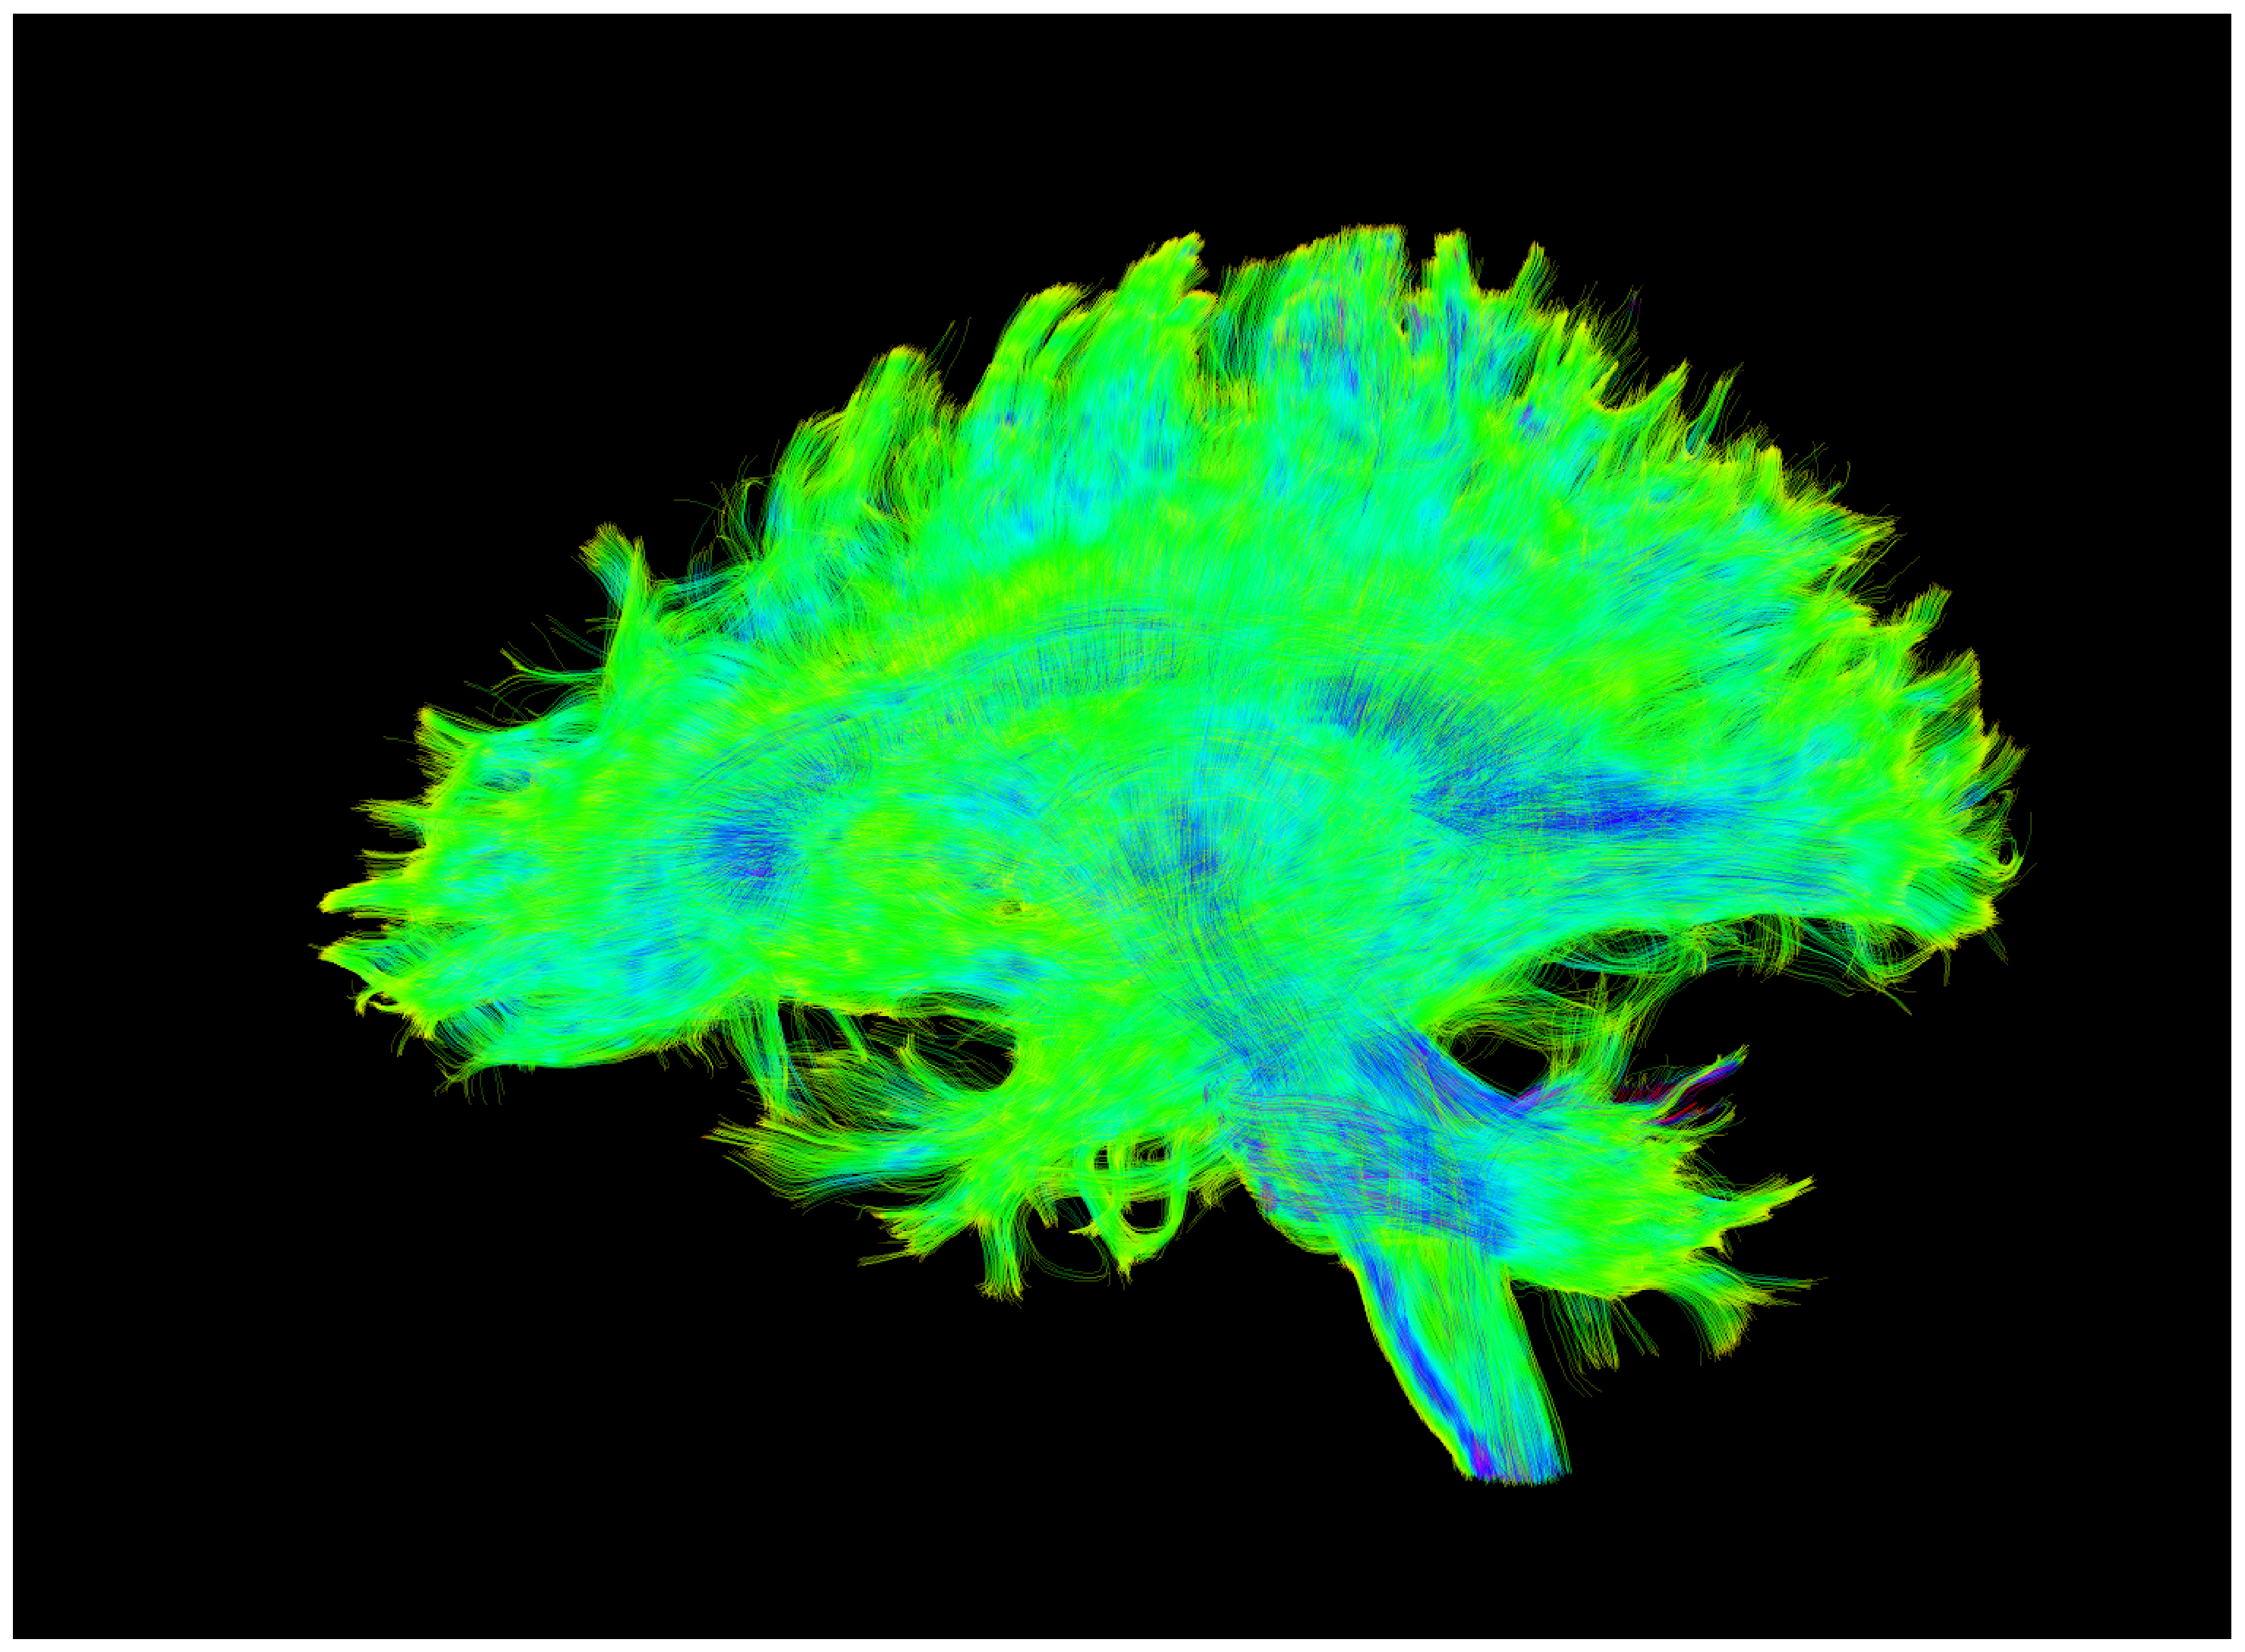
\includegraphics[width=4cm]{Tarctography1-Left-View}
        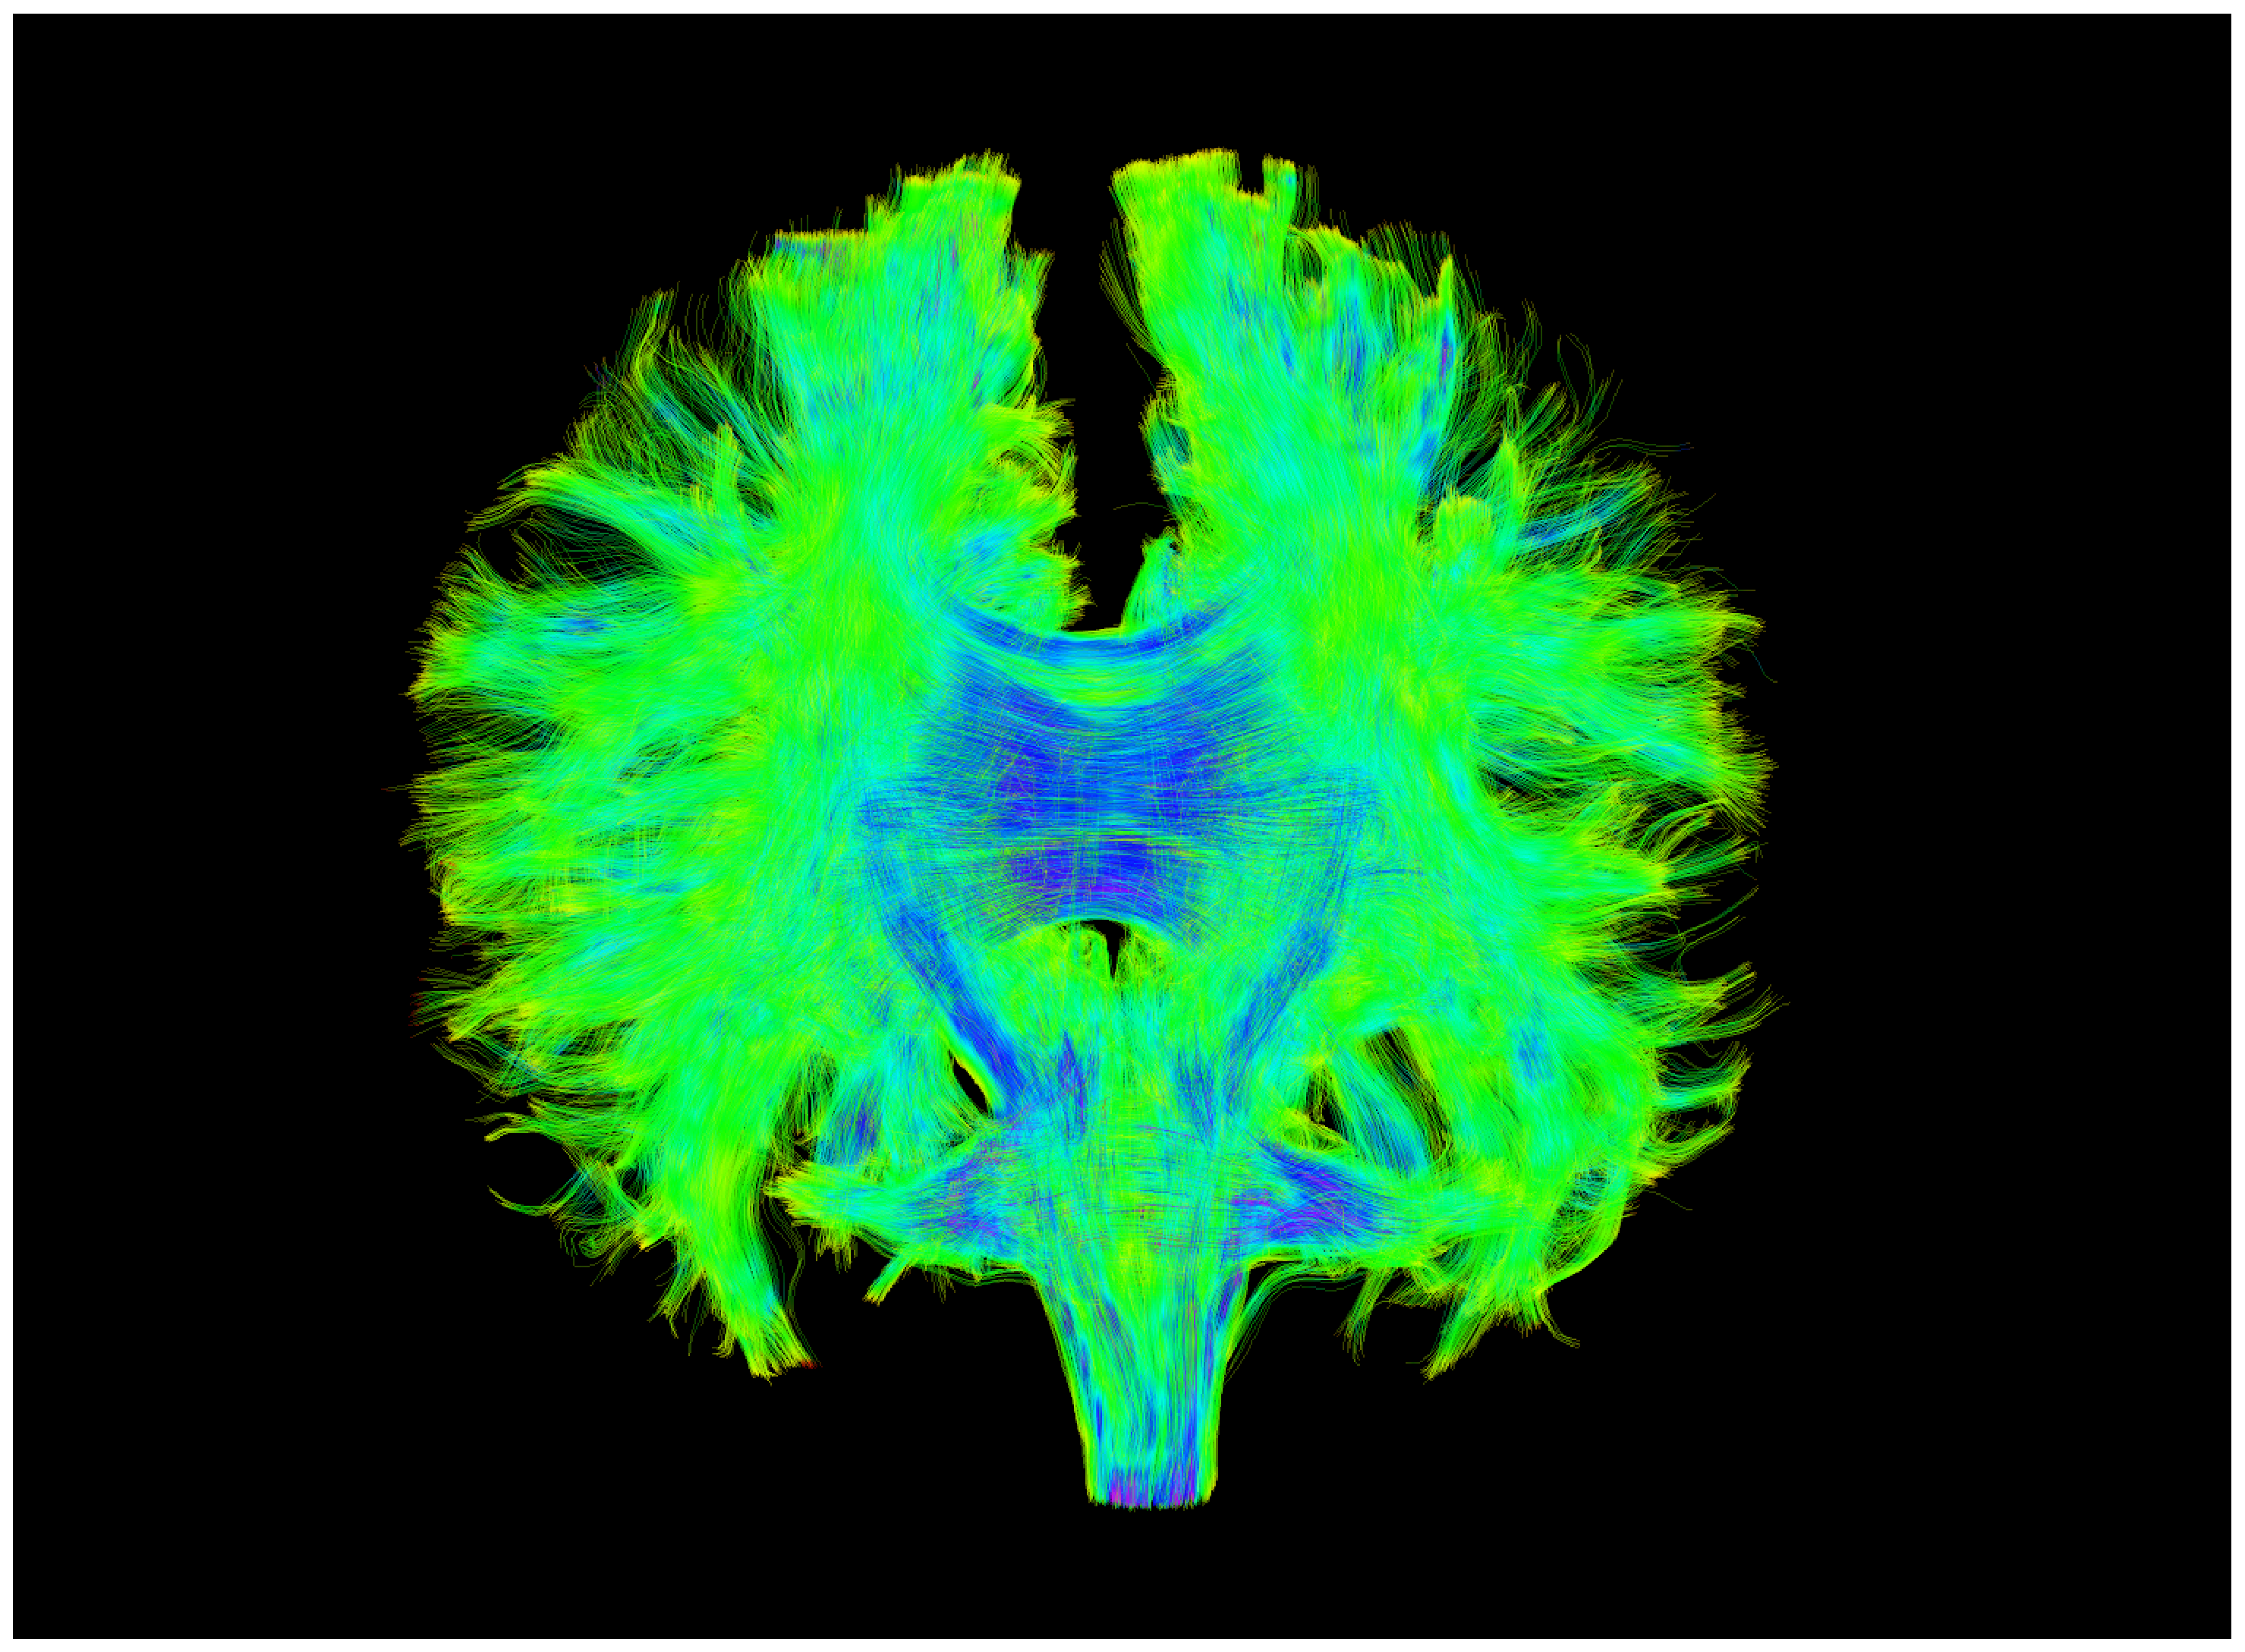
\includegraphics[width=4cm]{Tarctography1-Anterior-View}
        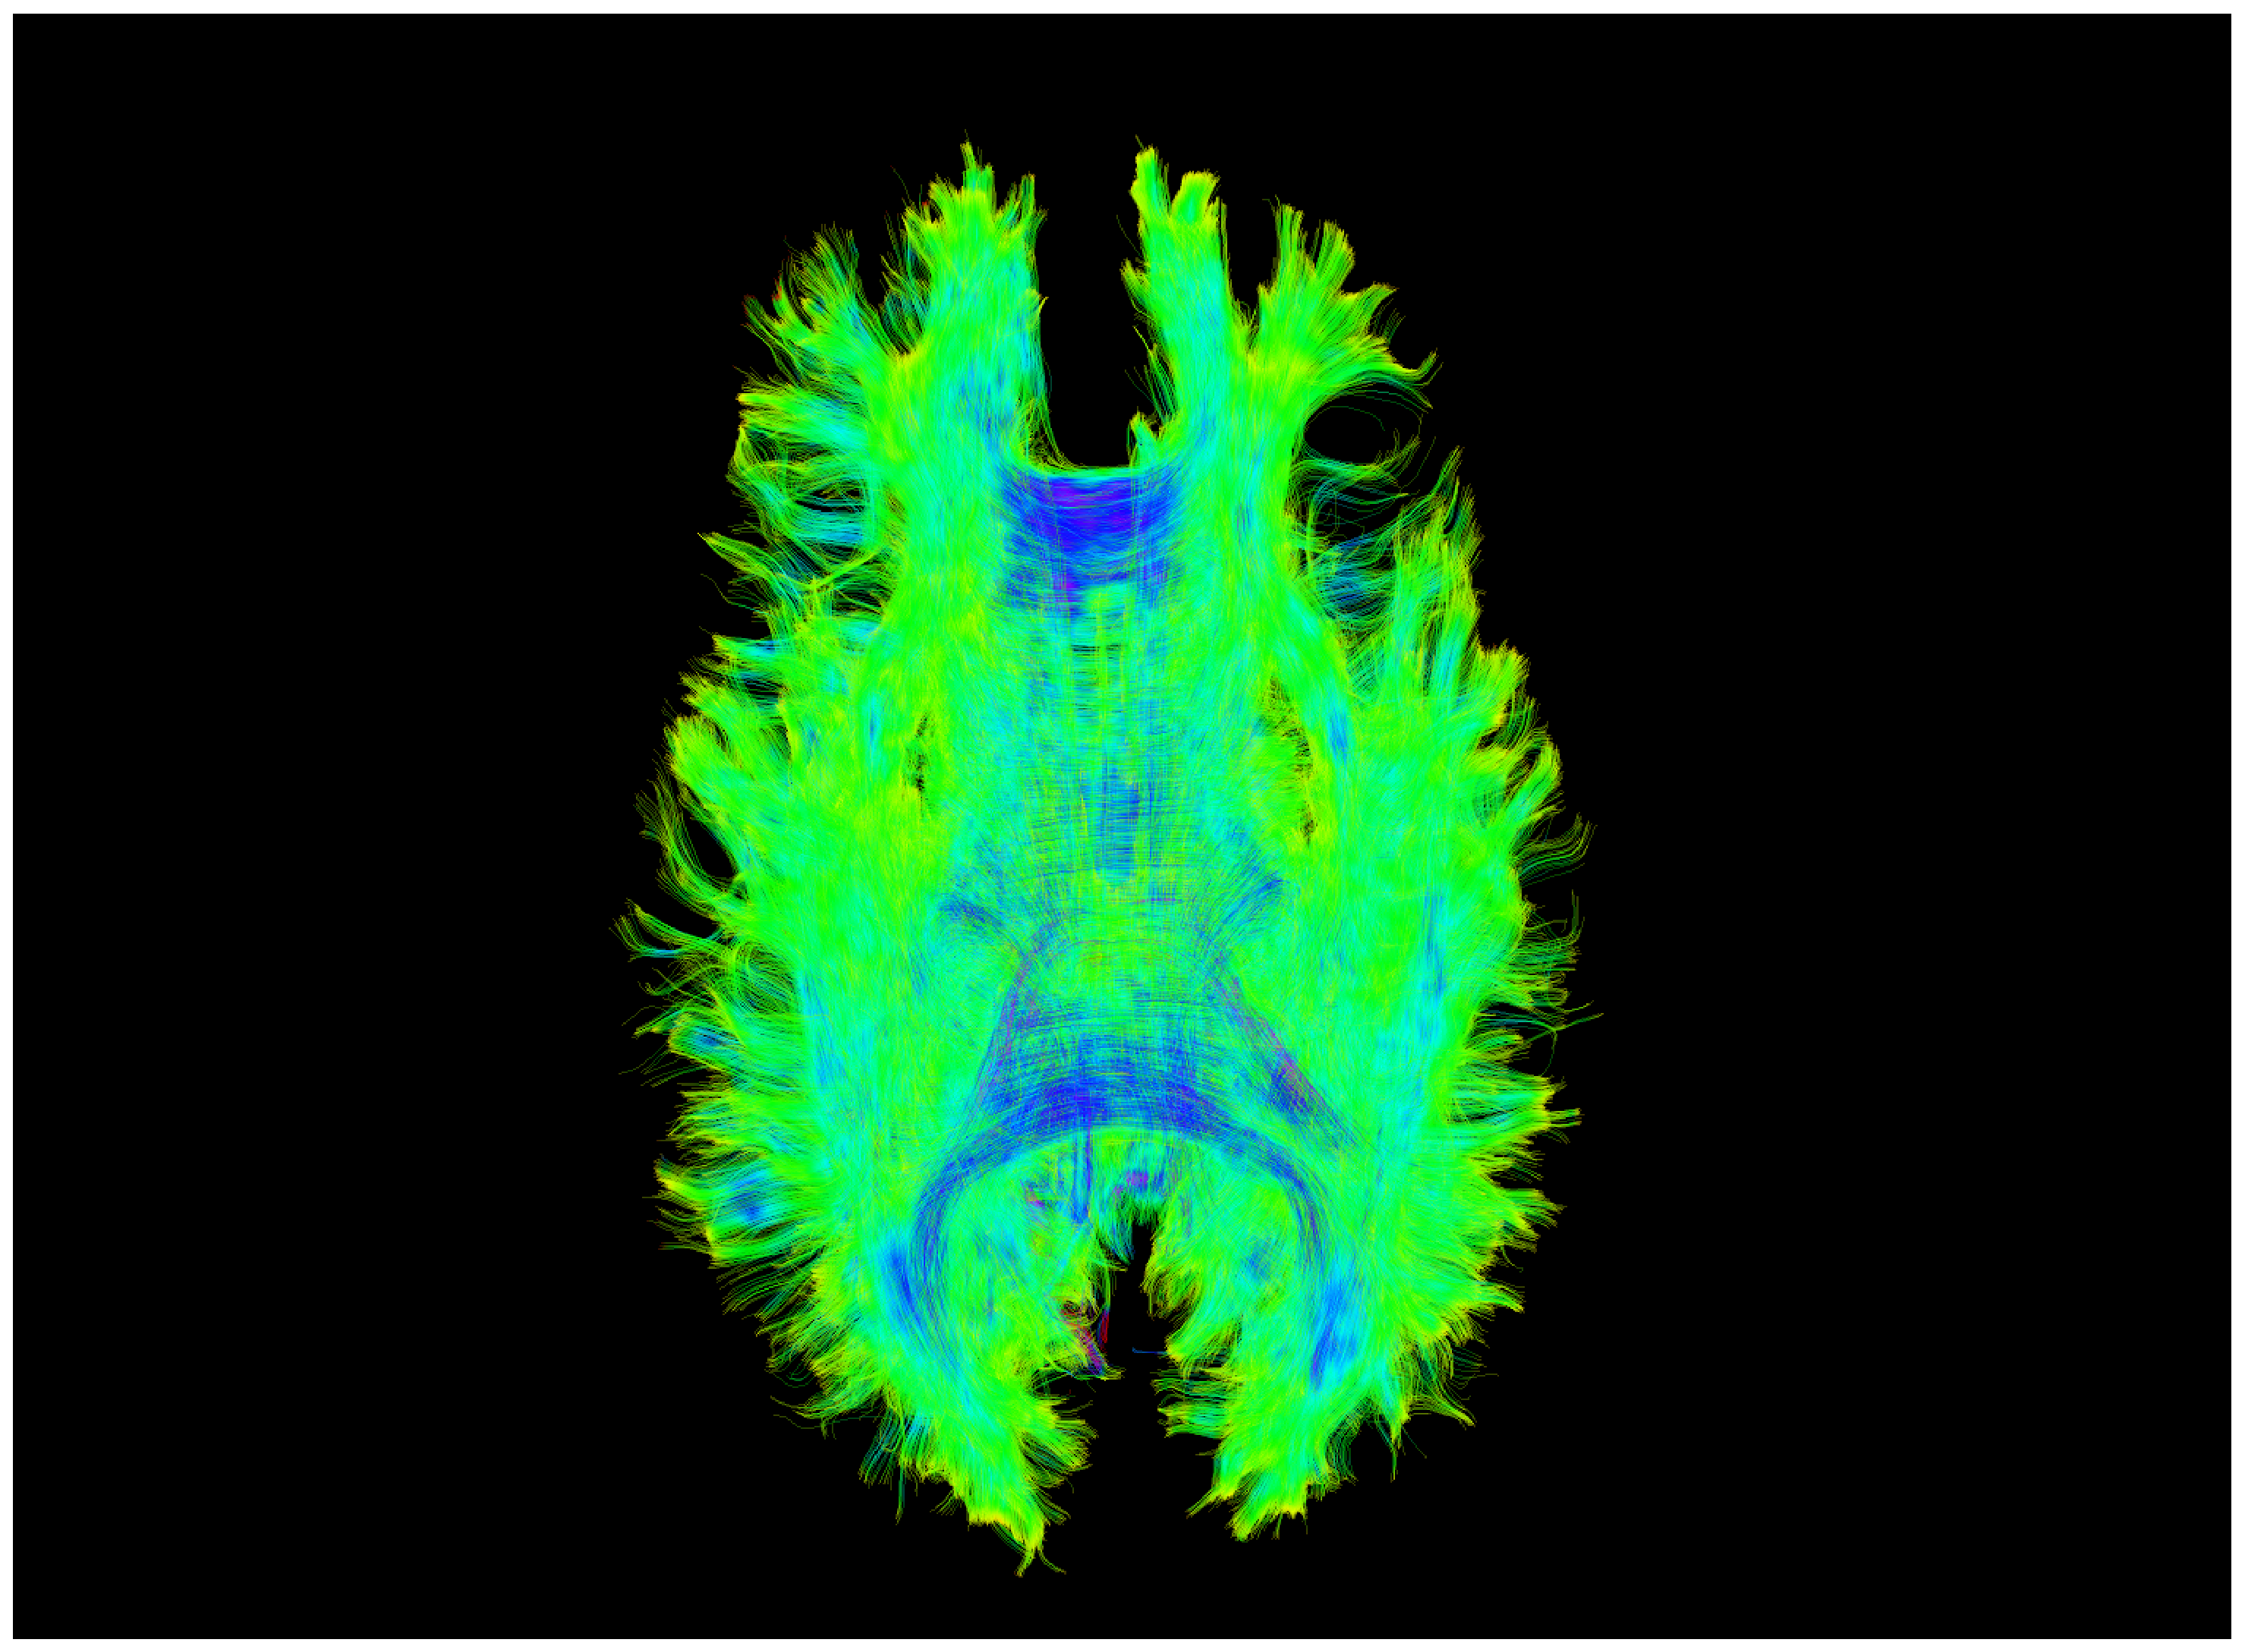
\includegraphics[width=4cm]{Tarctography1-Interior-View}

        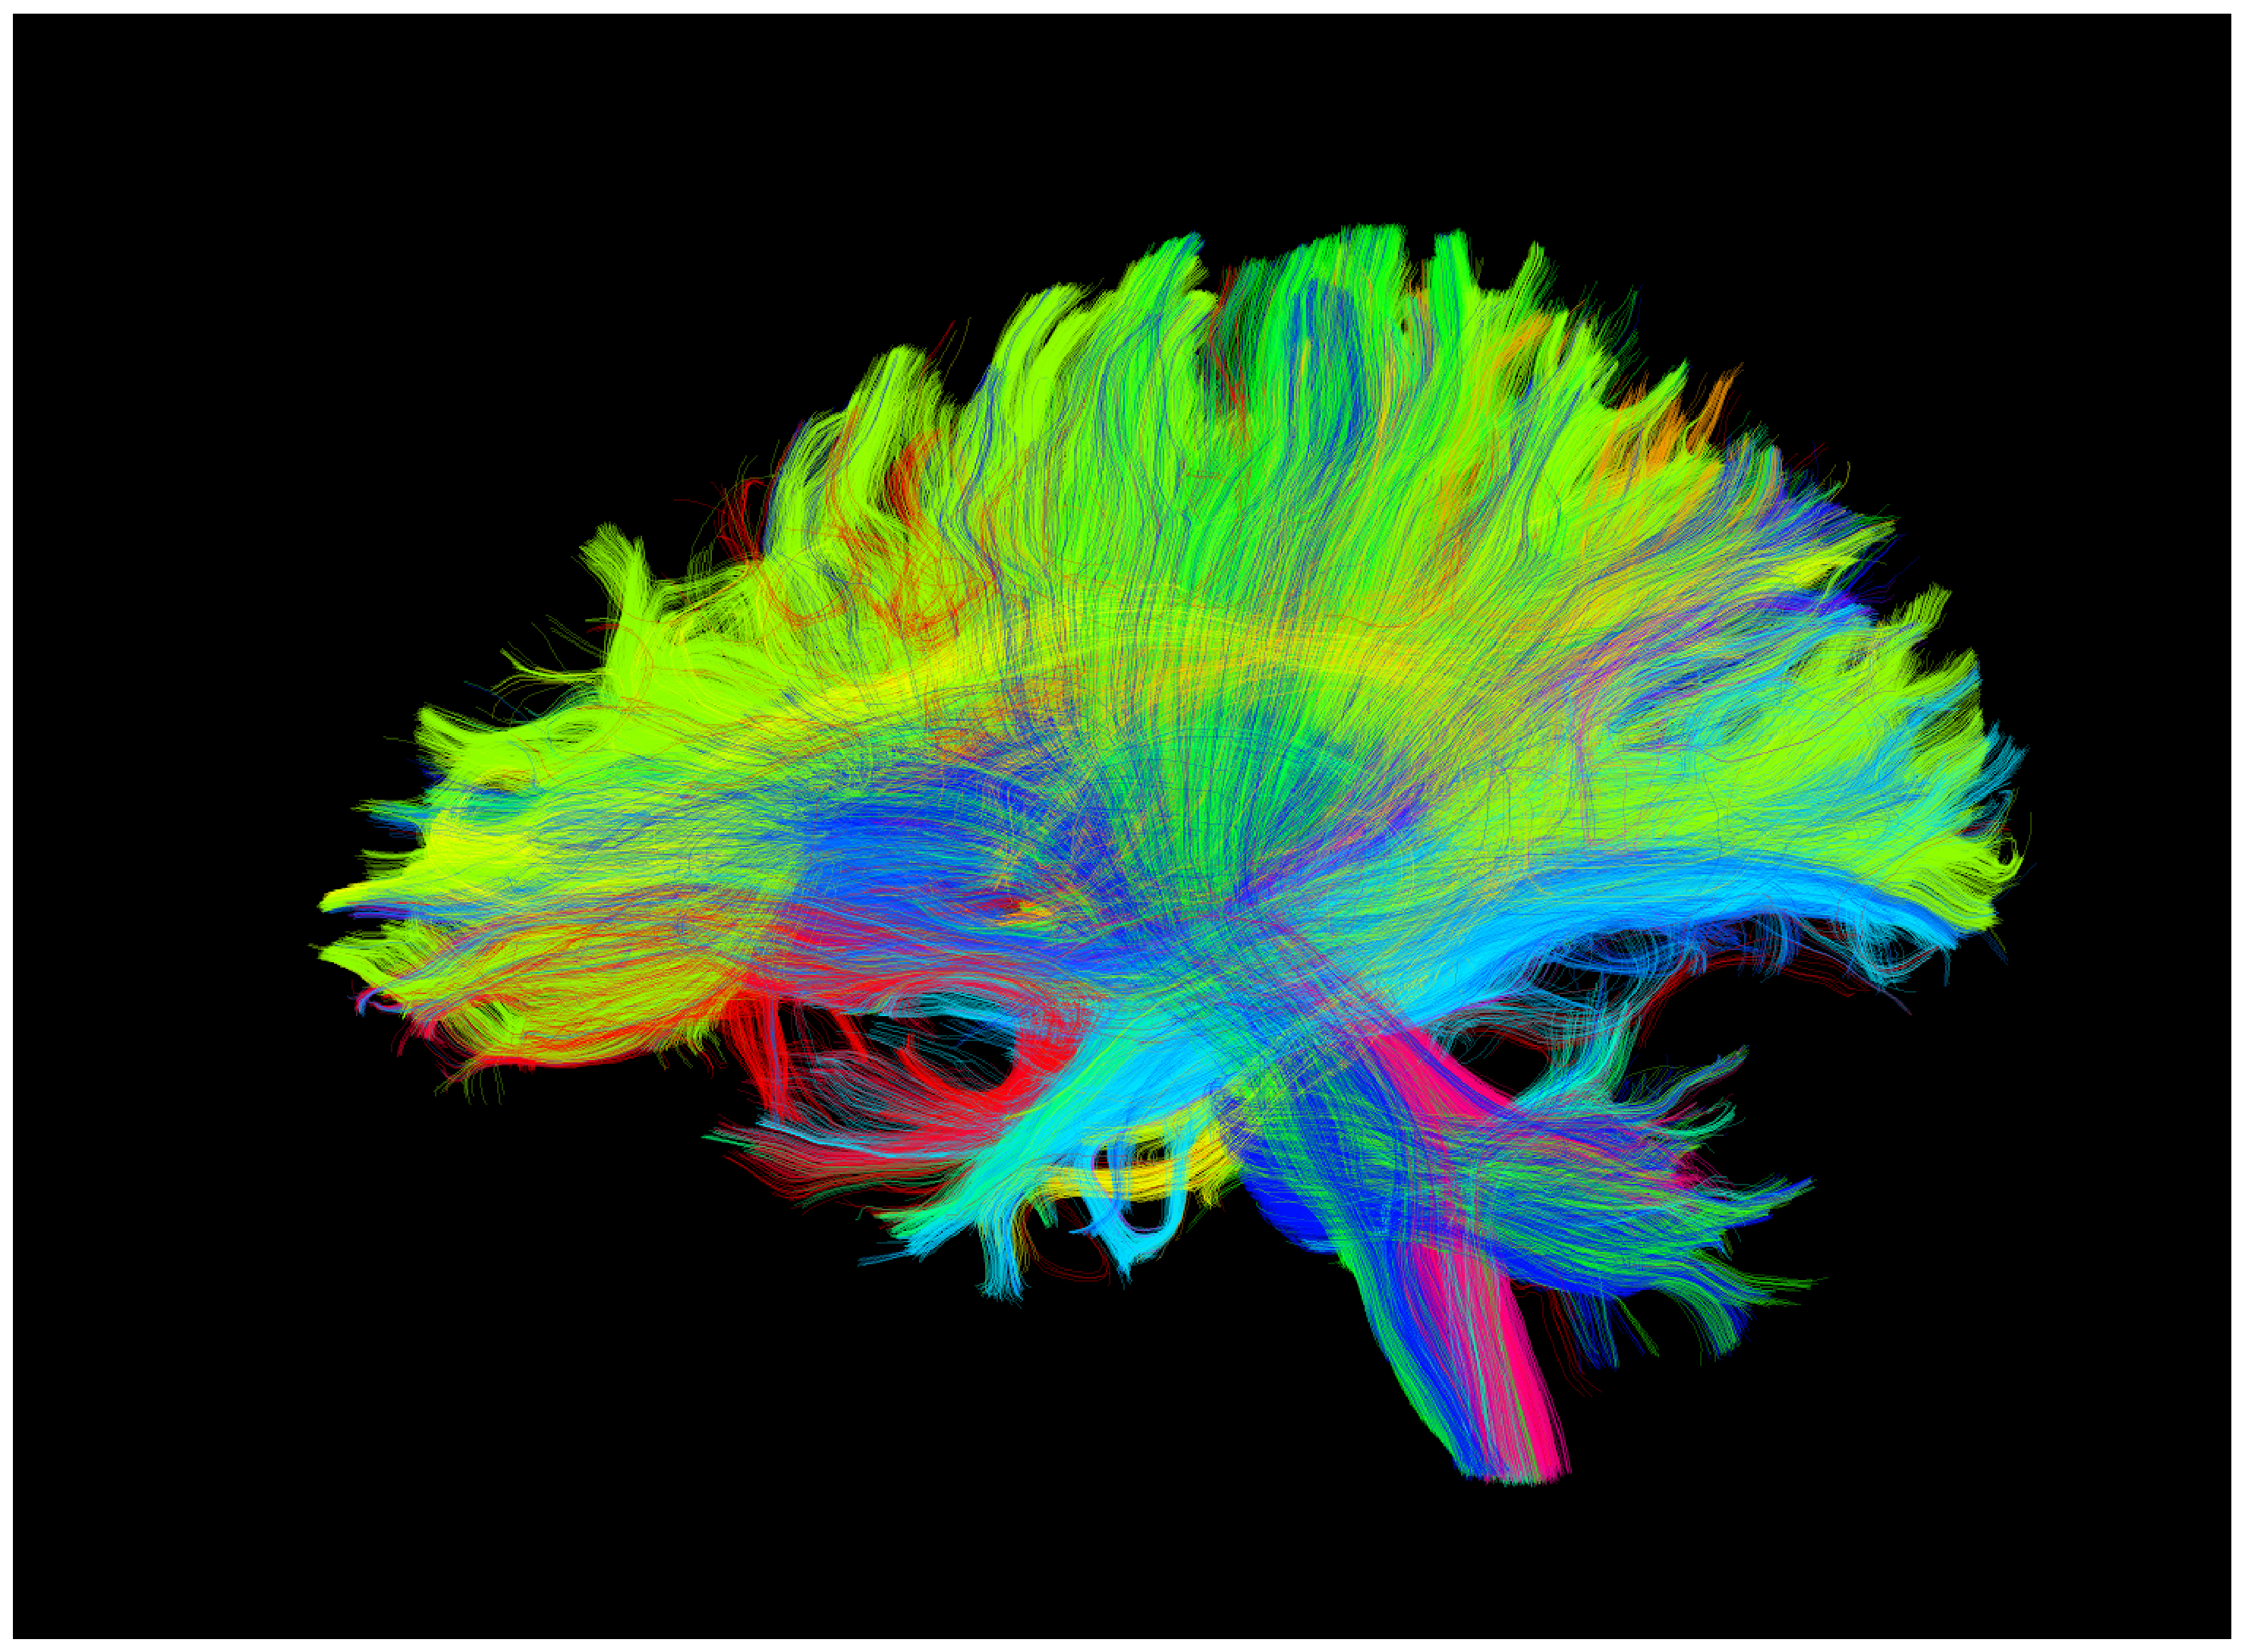
\includegraphics[width=4cm]{Clustering1-Left-View}
        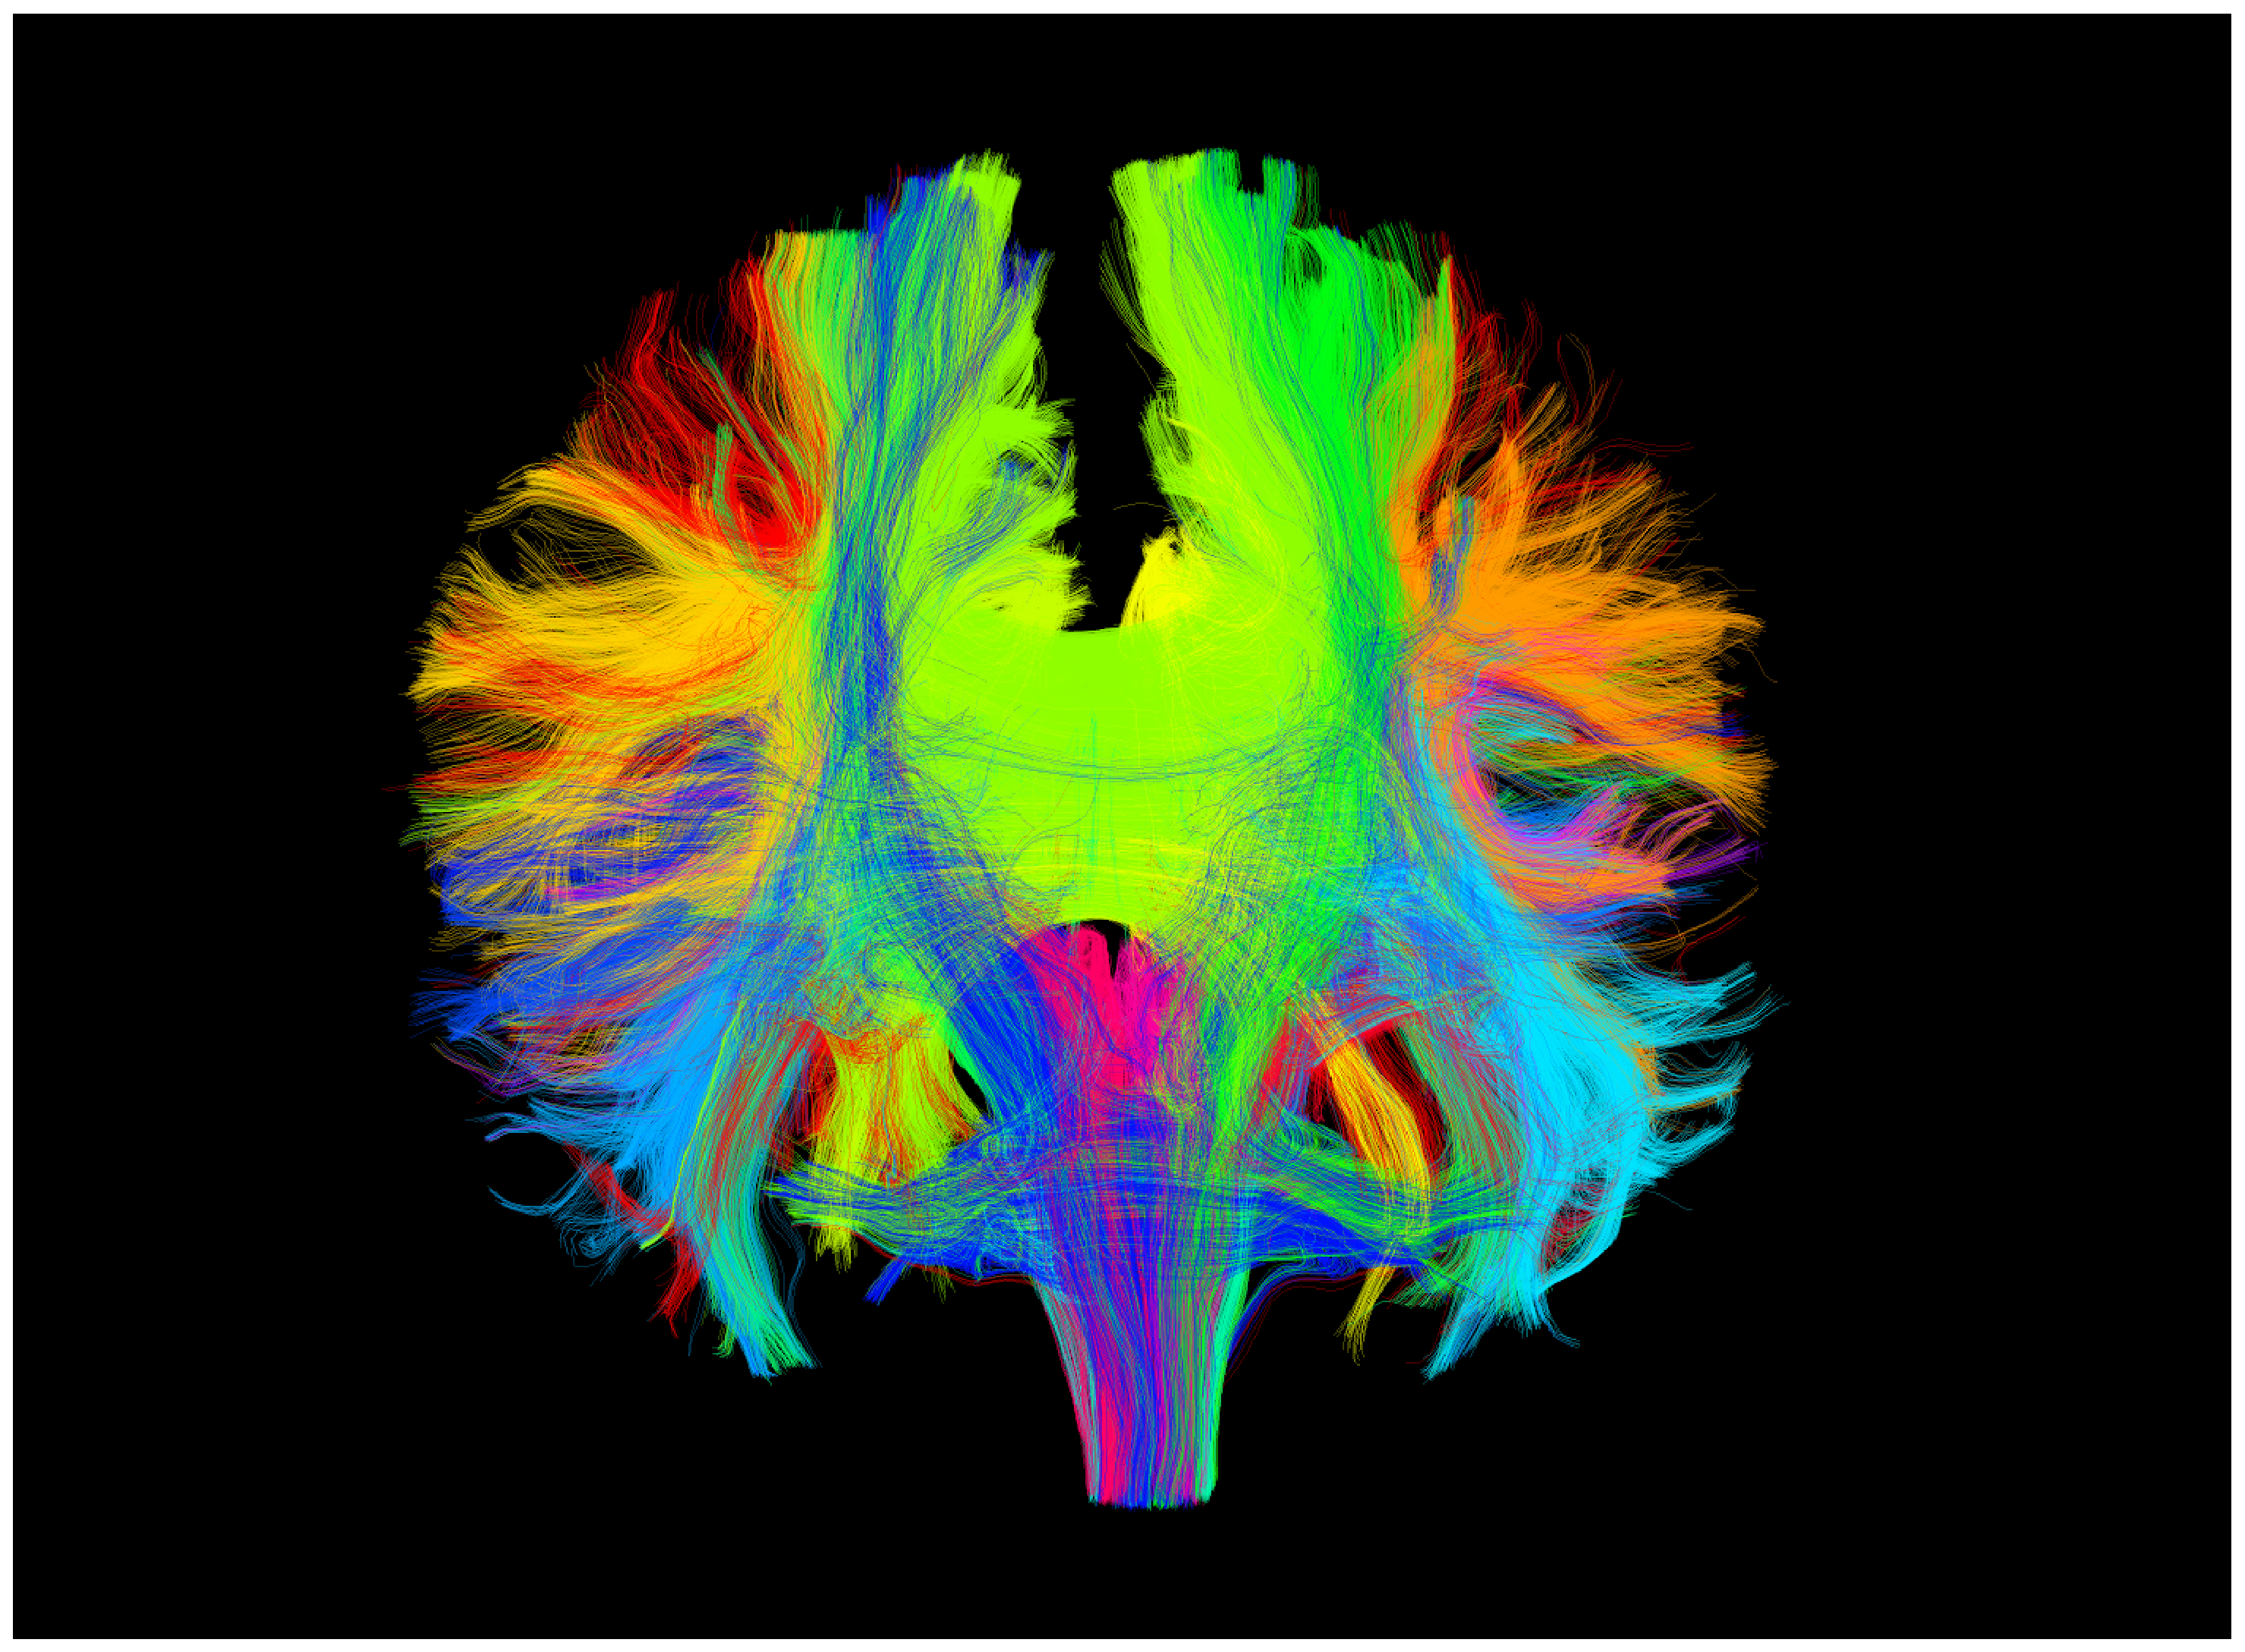
\includegraphics[width=4cm]{Clustering1-Anterior-View}
        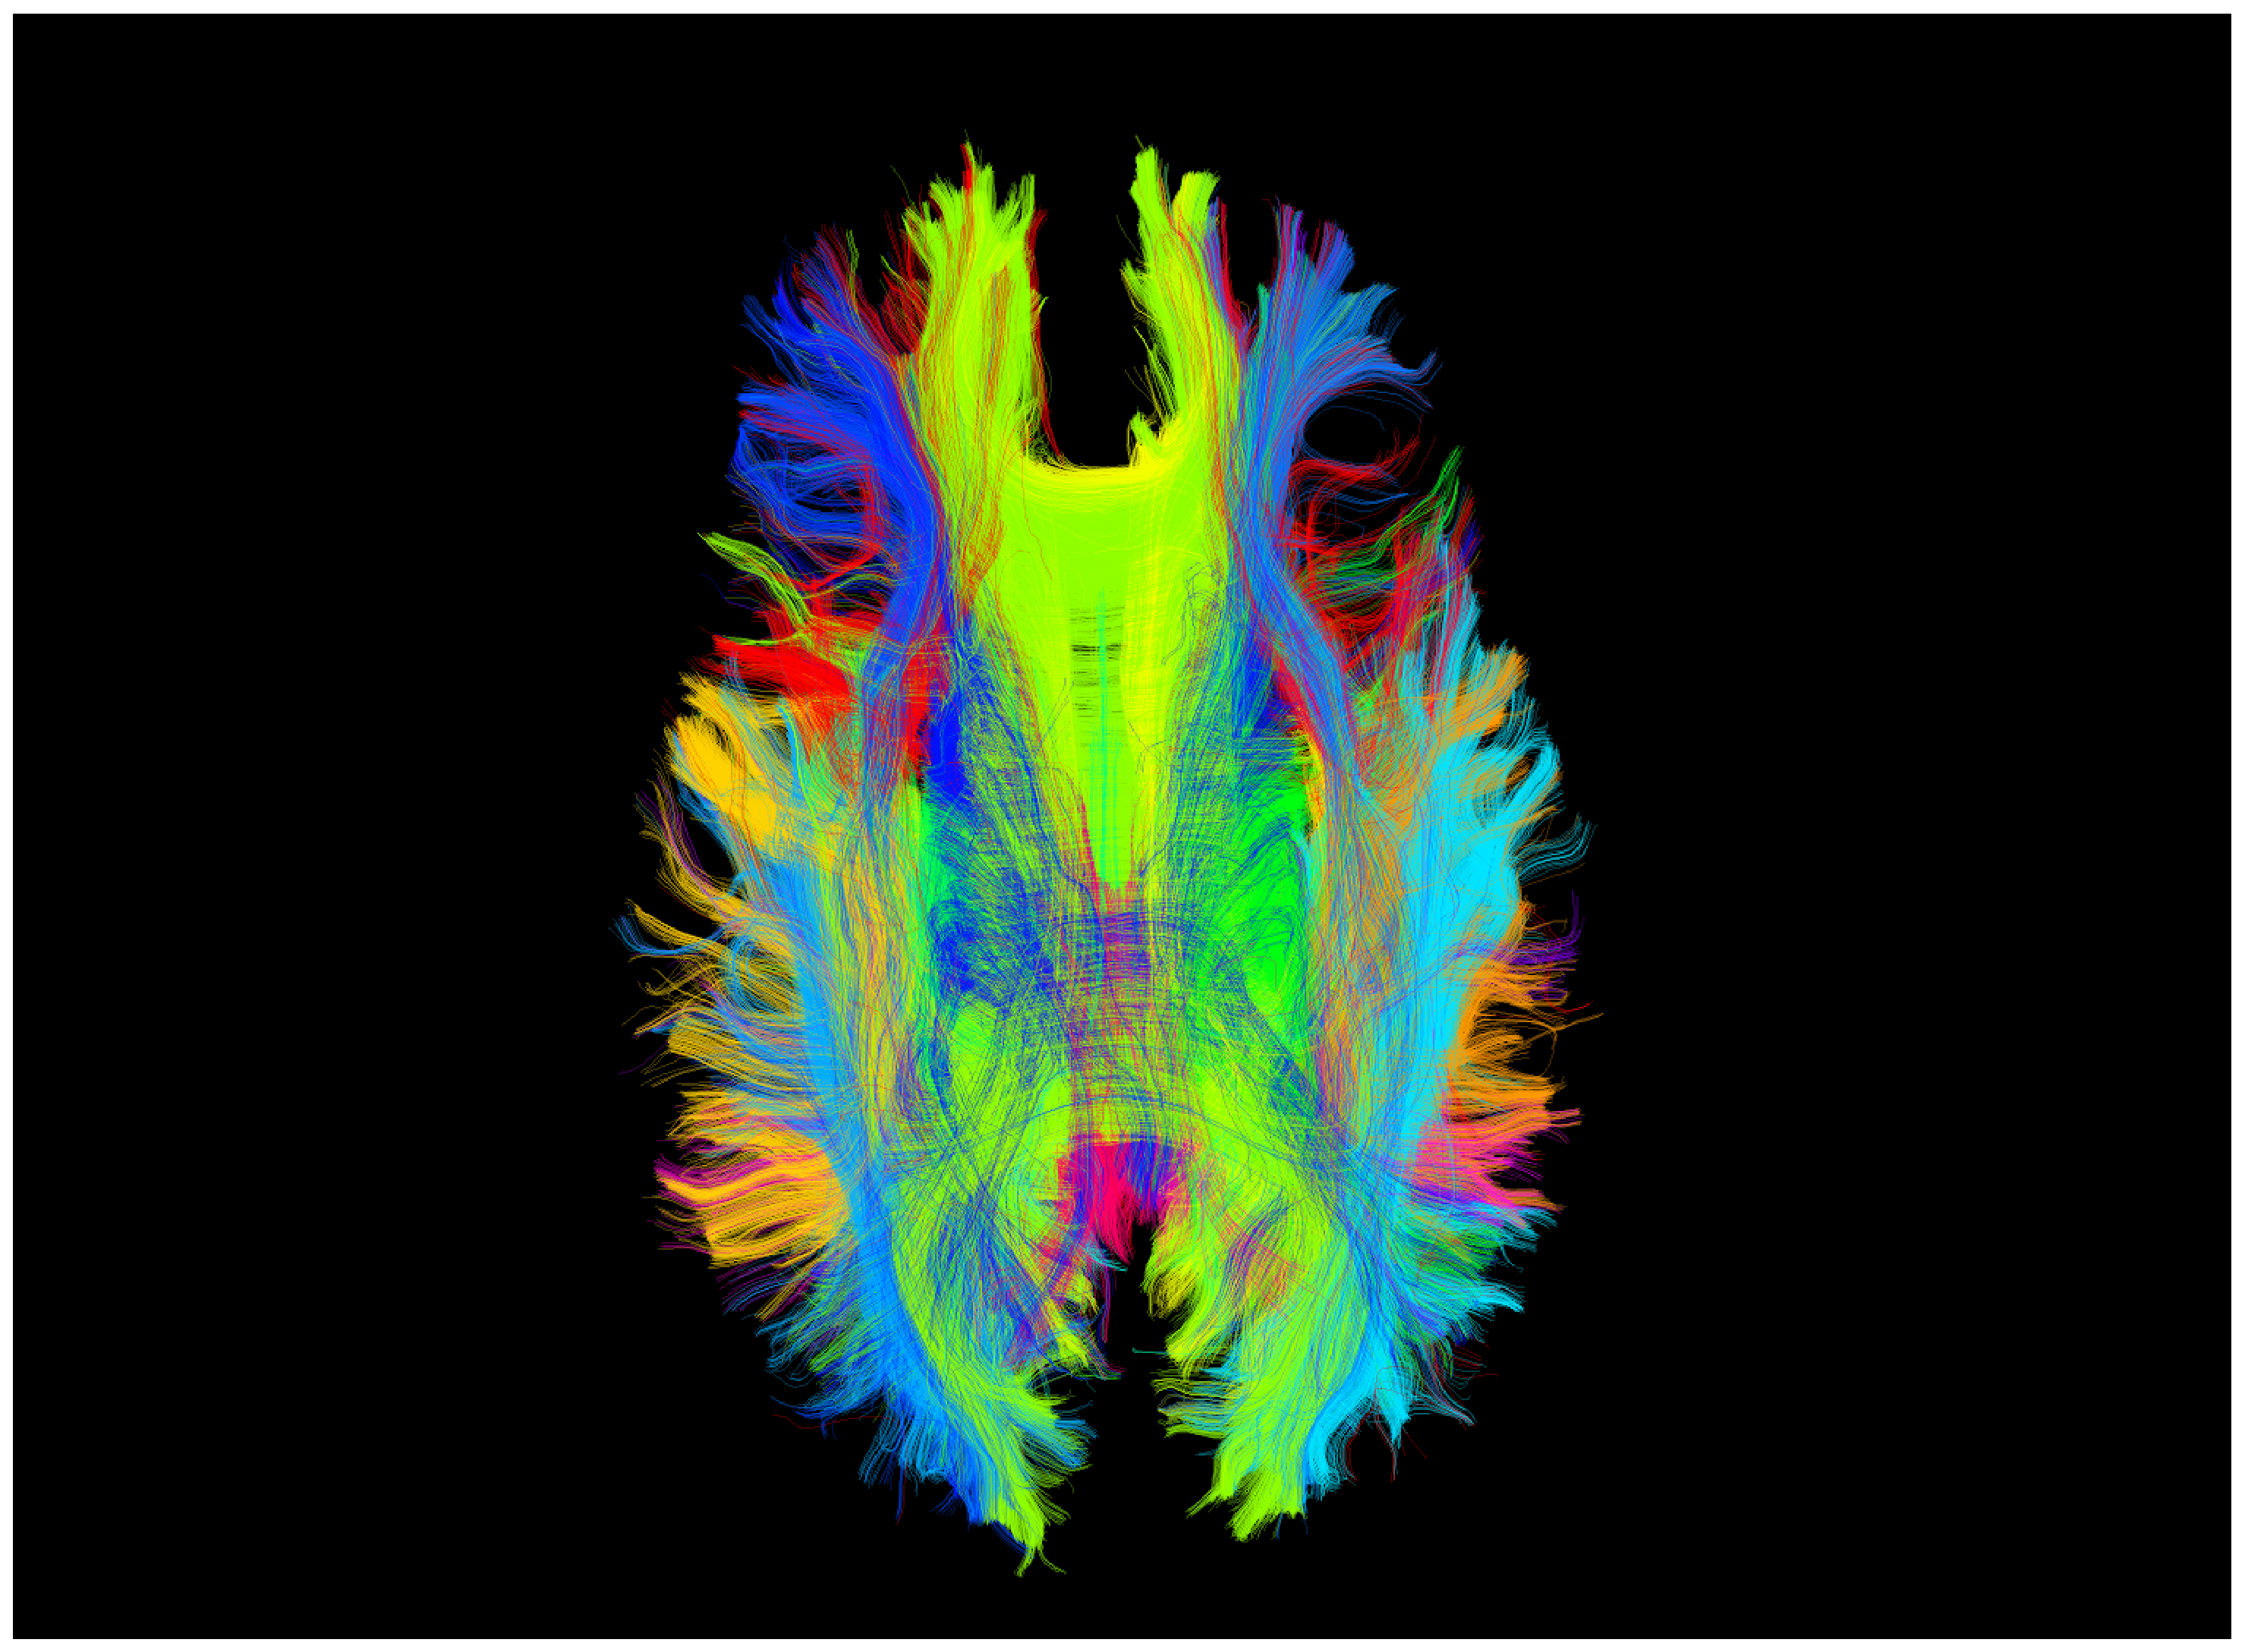
\includegraphics[width=4cm]{Clustering1-Interior-View}

        \caption{An example of fiber tracts clustering in the whole brain using \texttt{btkProbabilisticSegmentationMapBasedClustering} method.
        {\em The fibers from the tractography process and final clustering fiber bundles are shown in the first and second row, respectively. Three viewing angles of 3D depictions of fibers are shown (from left to right): left lateral view, anferior view and interior view. }}
        \label{clustering1-fig}
        \end{figure}

	\item[btkDistanceFibersKMeansApproximationClustering] ~\\

	Usage: \texttt{btkDistanceFibersKMeansApproximationClustering -b input.vtk -d distance\_measure -c number\_of\_clusters -a alpha -e eps -o output.vtk} \\

	Minimal usage: \texttt{btkDistanceFibersKMeansApproximationClustering -b input.vtk -d distance\_measure -c number\_of\_clusters -o output.vtk} \\

	The full list of optional parameters of this method can be obtained by:\\ 
        \texttt{btkDistanceFibersKMeansApproximationClustering --help}

	Fig.\ref{clustering2-fig} shows an example of clustering results in the corpus callosum region obtained using the method above with the following input parameters: \texttt{-d 10 -c 7}.

	\begin{figure}[h]
	\centering
        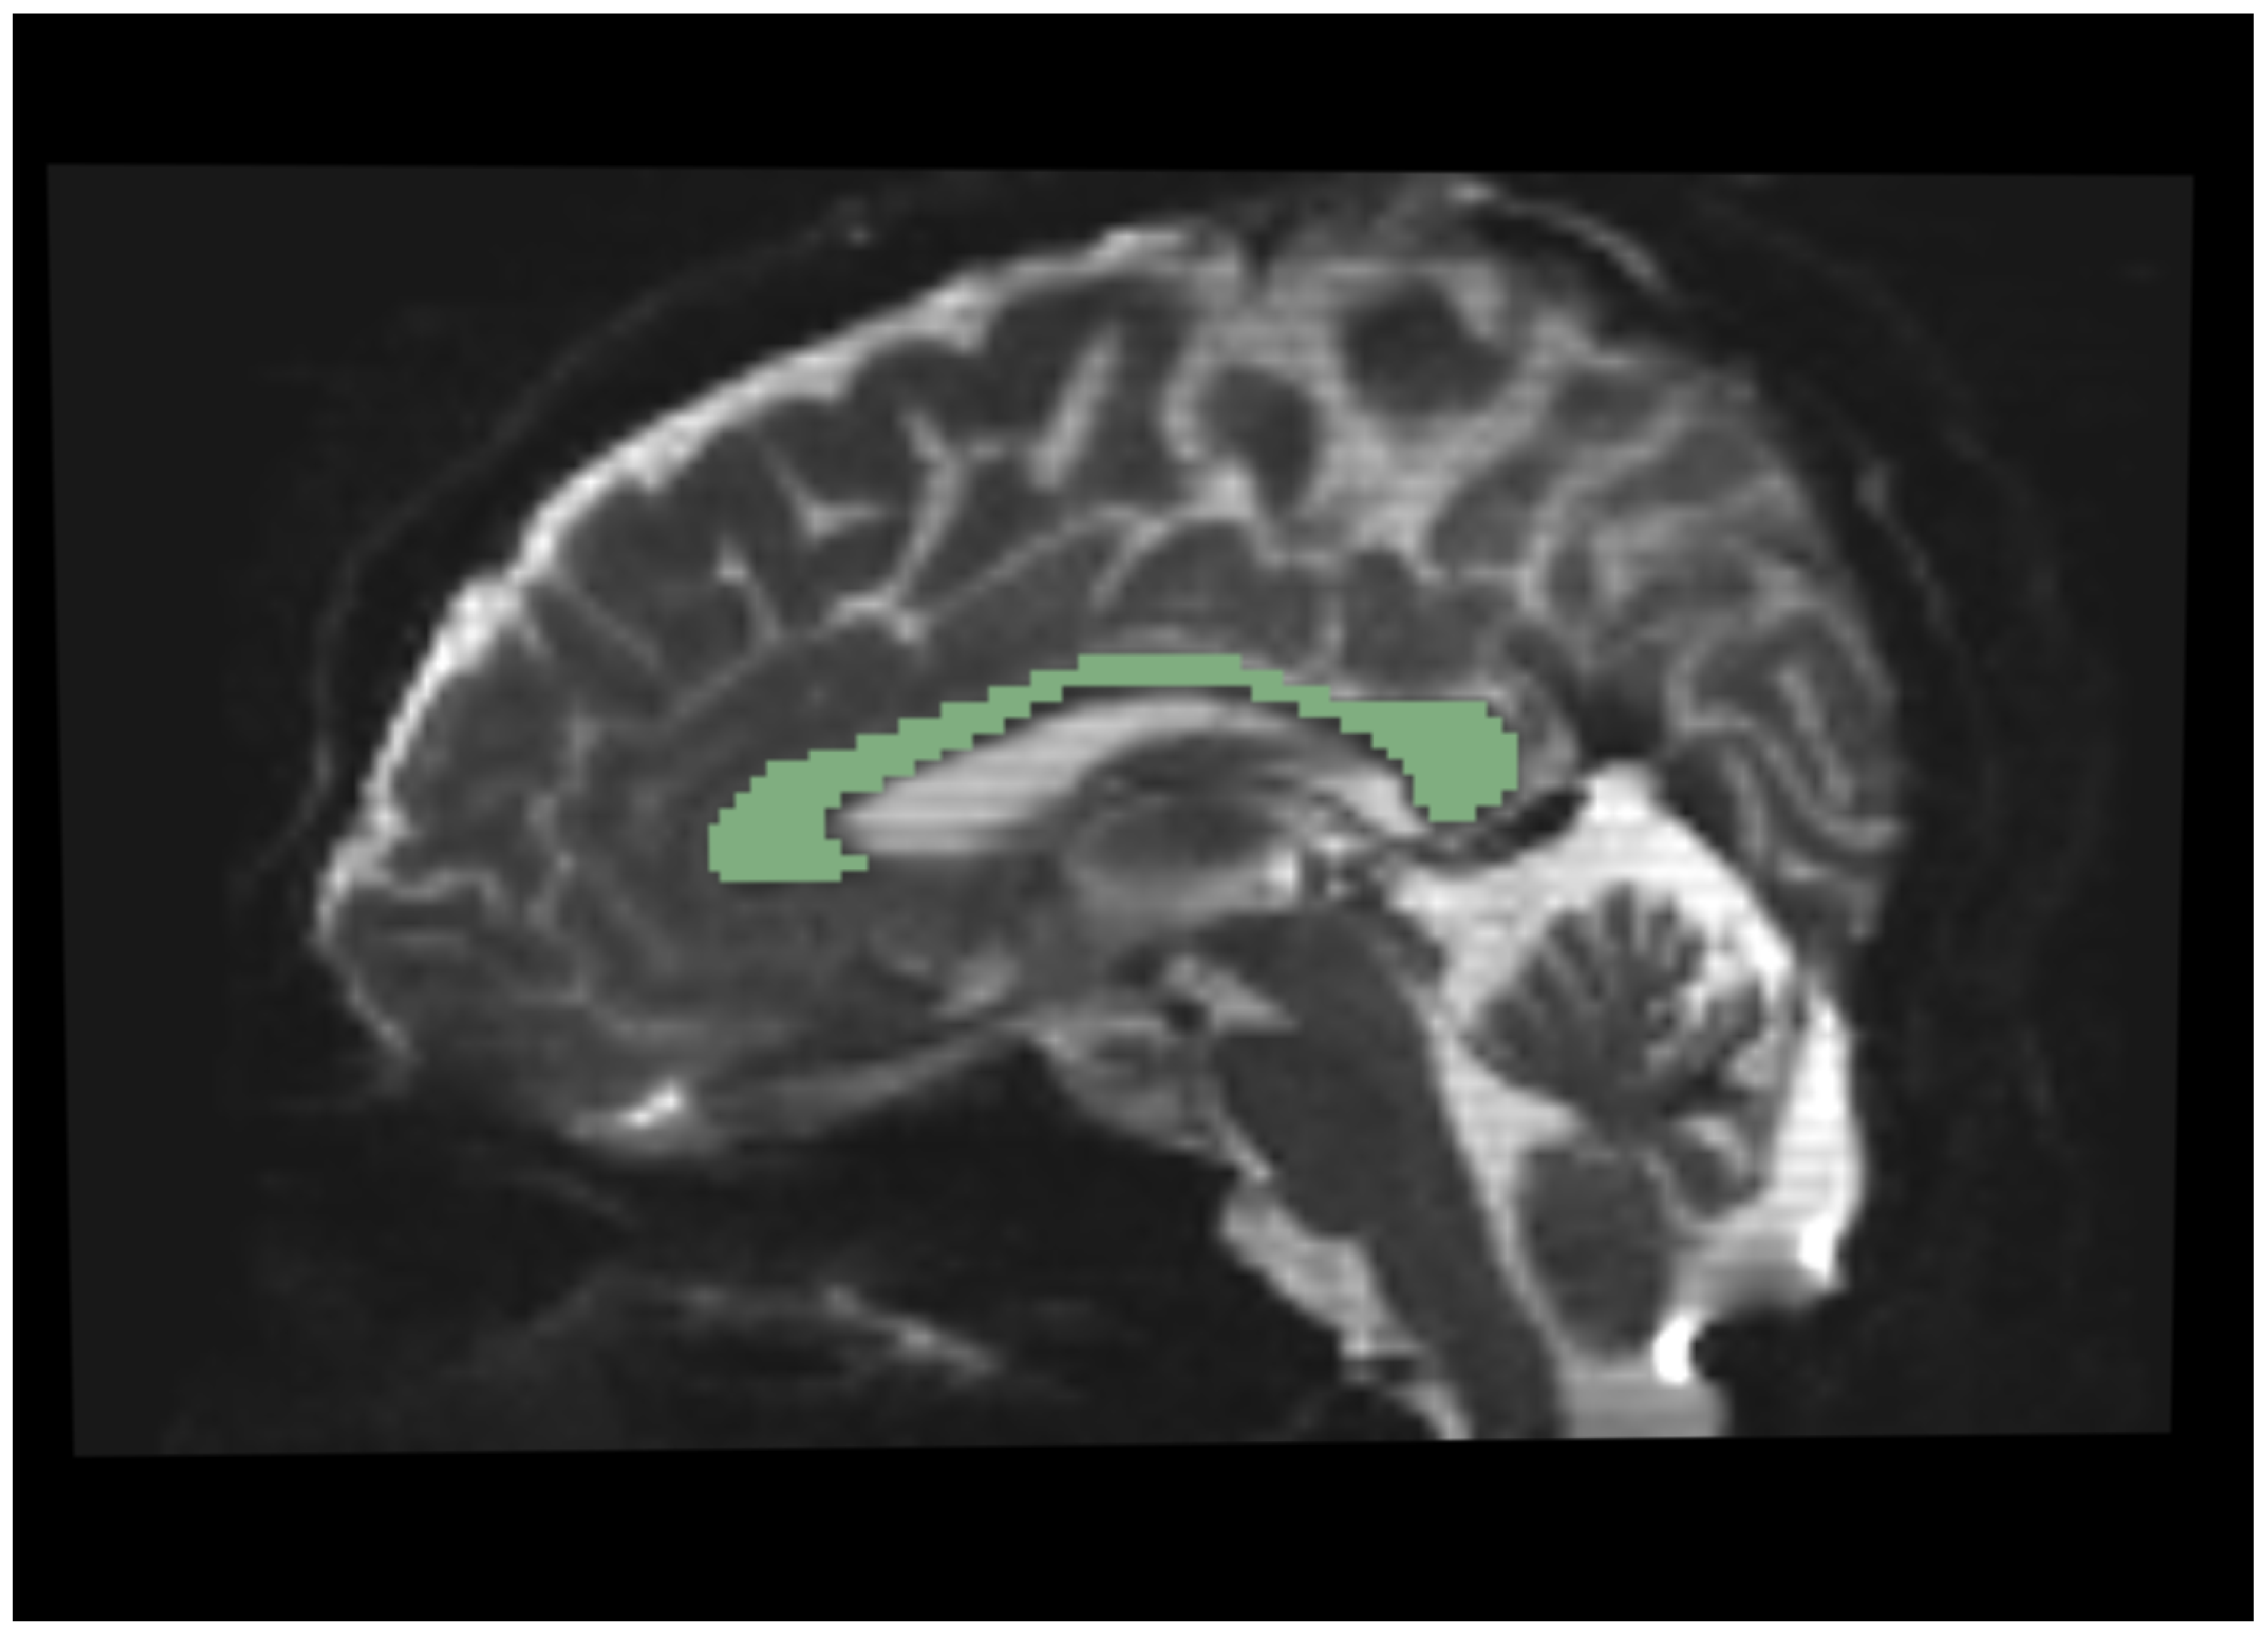
\includegraphics[width=4cm]{Corpus_Callosum-view2}
        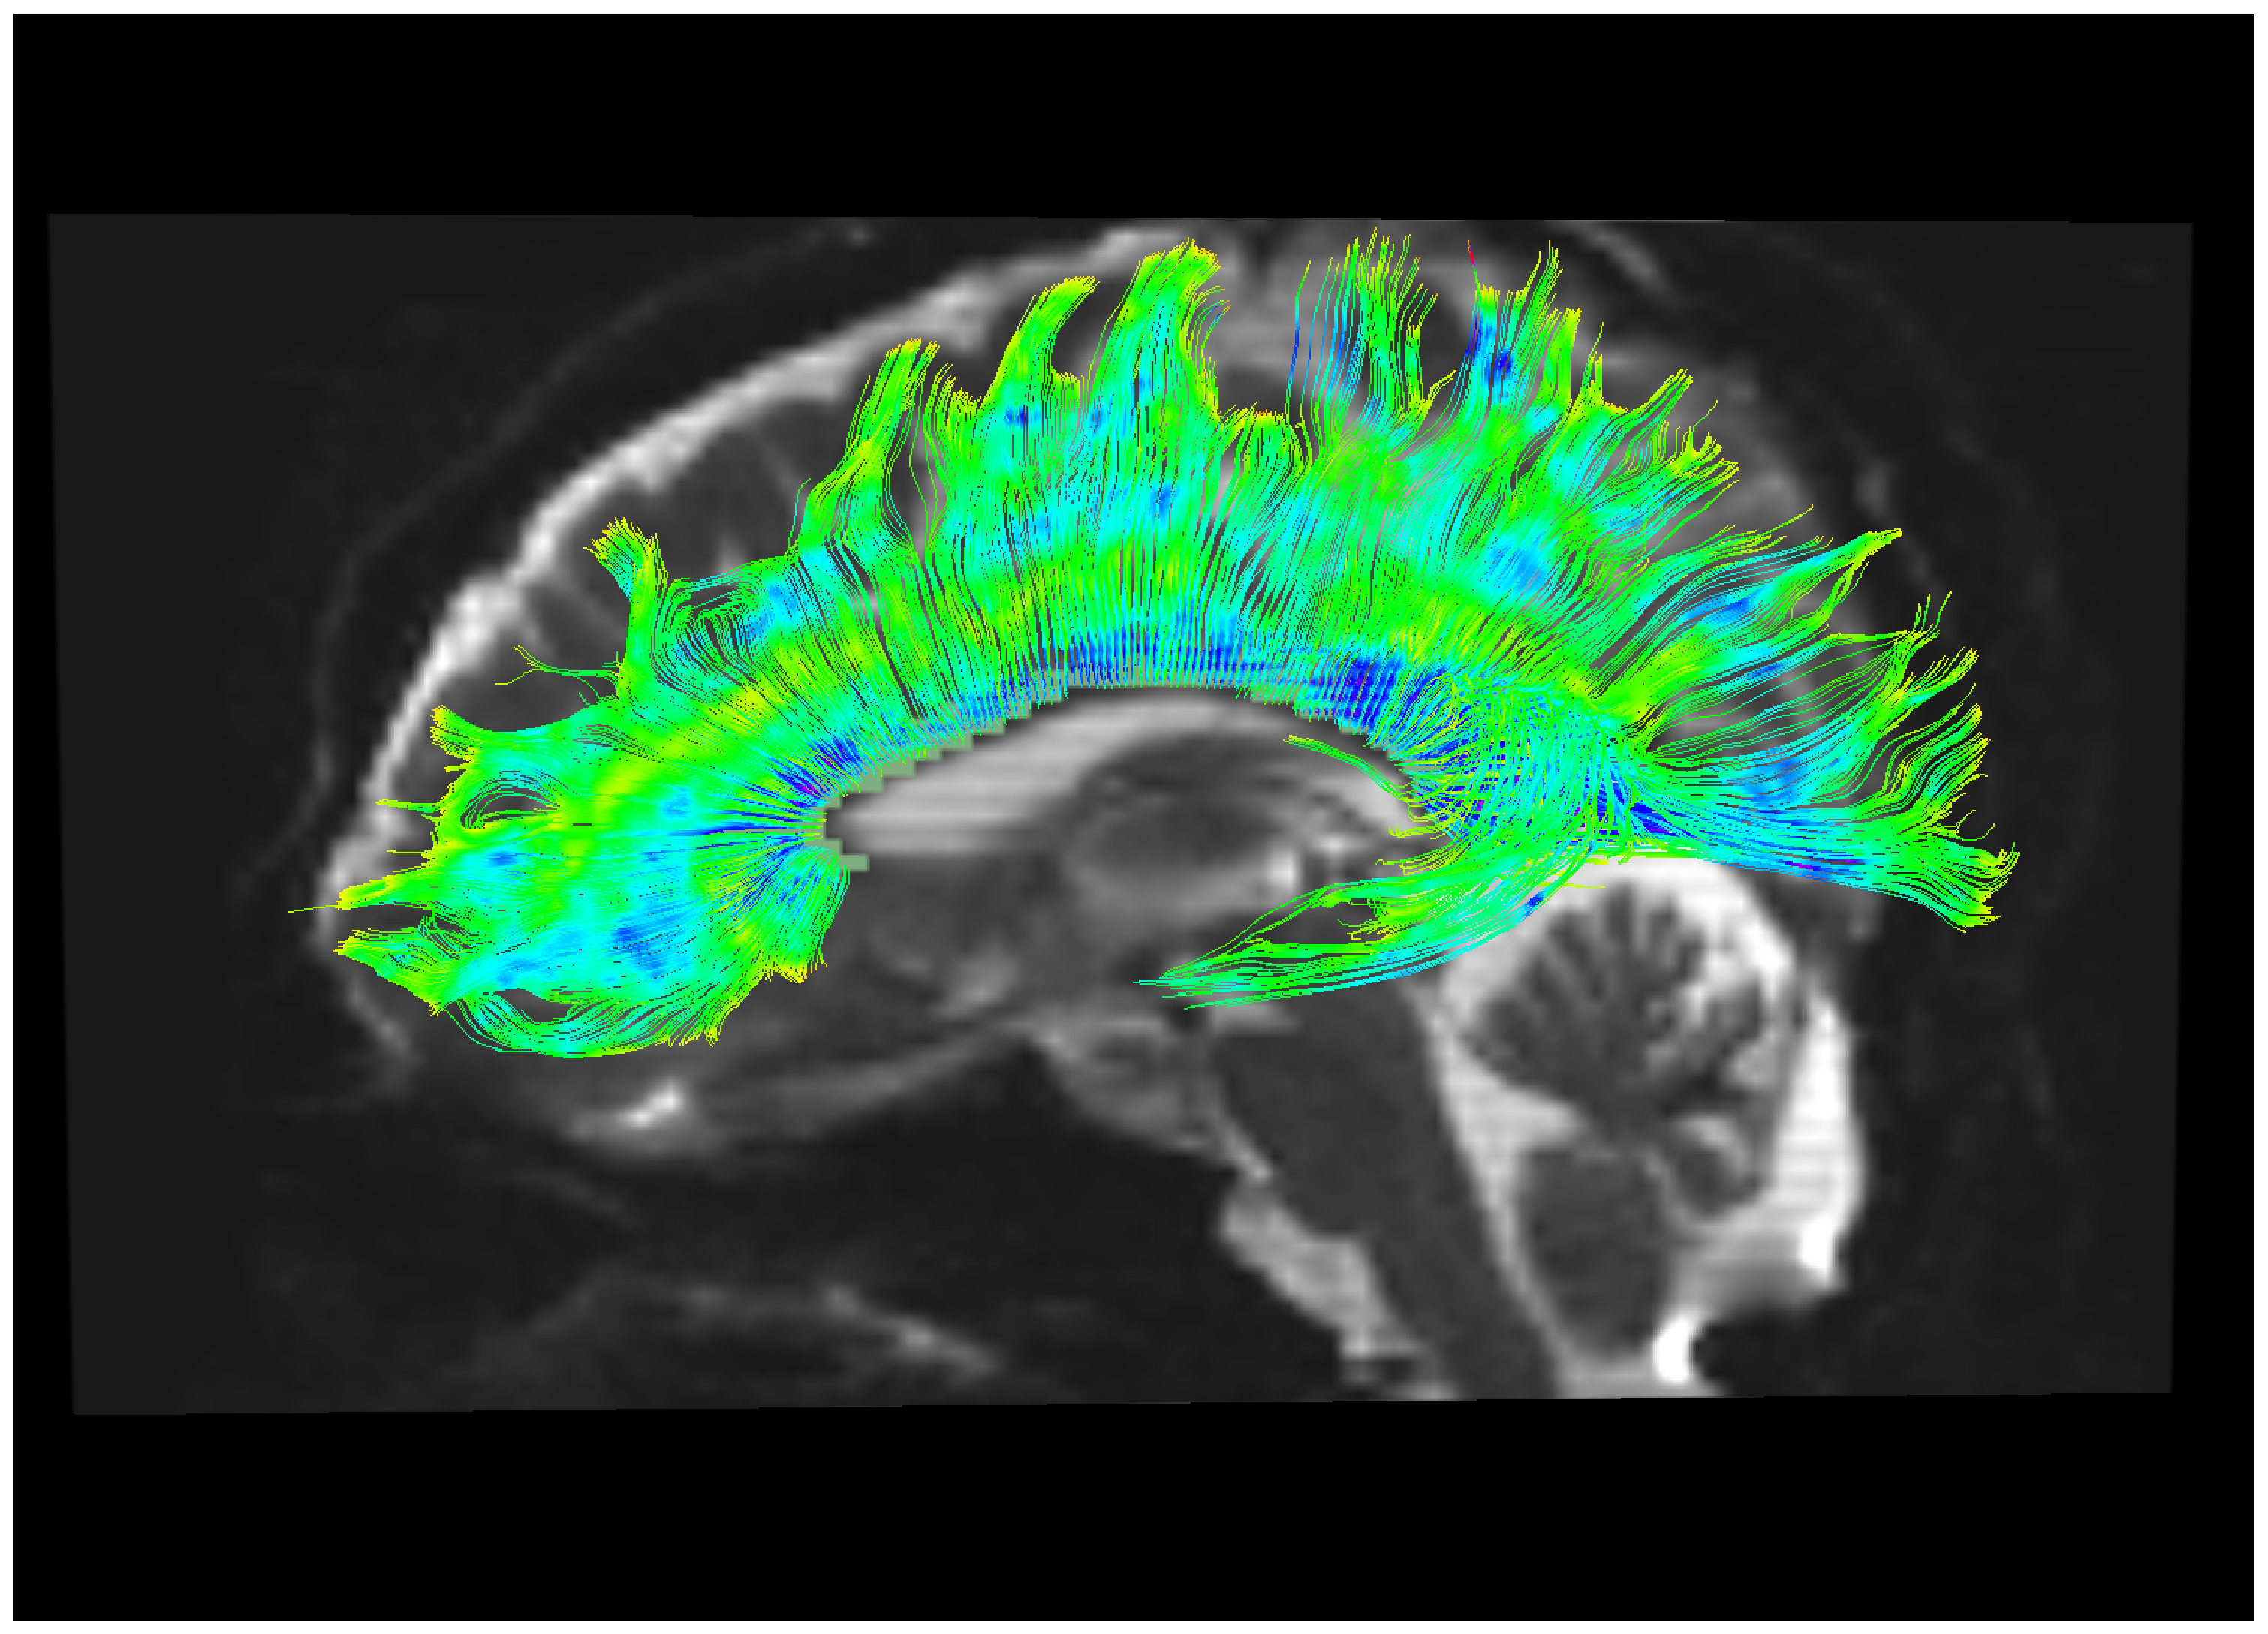
\includegraphics[width=4cm]{Tractography-CC-view2}
        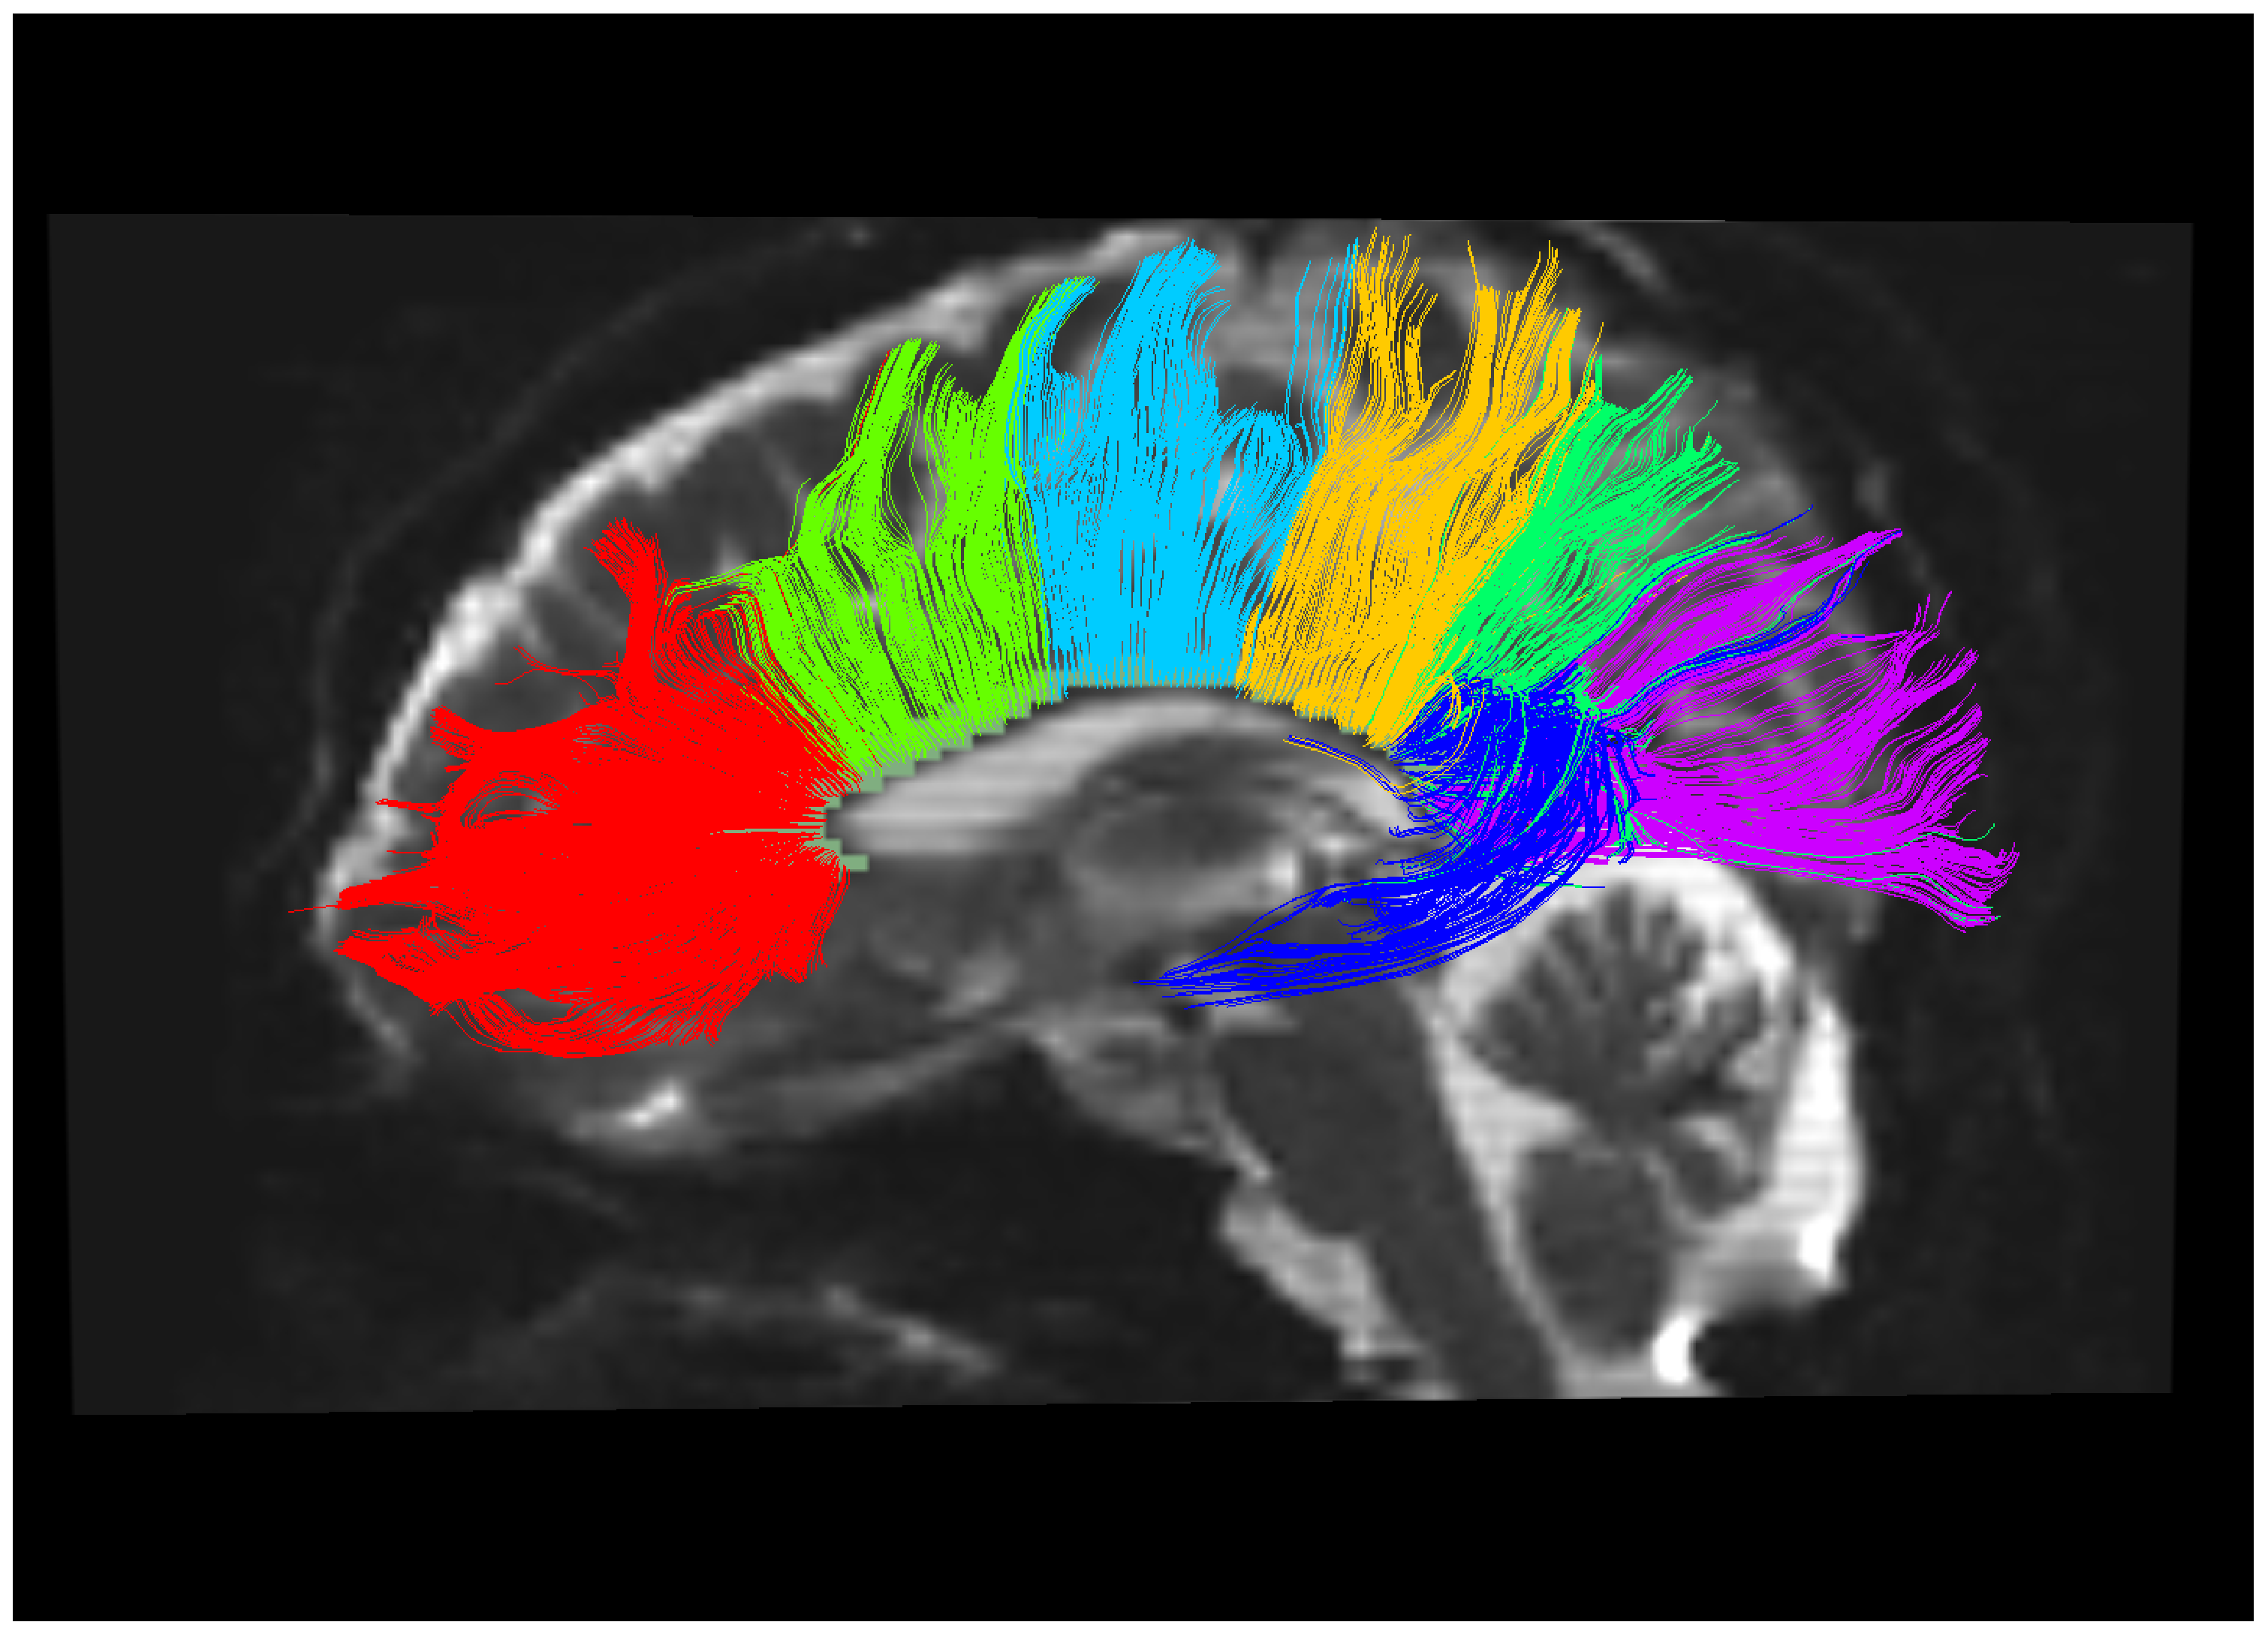
\includegraphics[width=4cm]{Clustering2-CC-view2}
        \caption{An example of fiber tracts clustering in the corpus callosum using \texttt{btkProbabilisticSegmentationMapBasedClustering} method.
        {\em The region of interest on the corpus callosum, fibers from the tractography process and final clustering fiber bundles are shown from left to right, respectively. The fibers are clustered according to anatomical regions as proposed by \href{brain.oxfordjournals.org/content/112/3/799}{Witelson}.}}
        \label{clustering2-fig}
        \end{figure}

\end{description}

\underline{NOTE}: The input and output data of these two applications are in \href{www.vtk.org/VTK/img/file-formats.pdf}{vtk} format.

\newpage
\section{Utilities}
\label{sec:utilities}

\begin{description}

%------------------------------------------------------------------------------
\addcontentsline{toc}{subsection}{btkApplyMaskToImage}
\item[btkApplyMaskToImage]: Multiply an image with a mask.
%------------------------------------------------------------------------------
\addcontentsline{toc}{subsection}{btkApplyTransformationToImage}
\item[btkApplyTransformationToImage]: Resample an image using a reference and a transformation (itk or btk).
%------------------------------------------------------------------------------
\addcontentsline{toc}{subsection}{btkAverage3DImages}
\item[btkAverage3DImages]: Compute the mean (and variance) image of a set of 3D images.
%------------------------------------------------------------------------------
\addcontentsline{toc}{subsection}{btkAverageImagesWithReference}
\item[btkAverageImagesWithReference]: Creates a high resolution image from a set of low resolution images.
%------------------------------------------------------------------------------
\addcontentsline{toc}{subsection}{btkBinarizeLabels}
\item[btkBinarizeLabels]: Binarize one label image (depending on the label value chosen).
%------------------------------------------------------------------------------
\addcontentsline{toc}{subsection}{btkBinarizeMask}
\item[btkBinarizeMask]: Binarize a float image using a threshold.
%------------------------------------------------------------------------------
\addcontentsline{toc}{subsection}{btkBinarizeTissueProbabilityMaps}
\item[btkBinarizeTissueProbabilityMaps]: Binarize a set of probability maps ([0,1]) into a short image (by taking the max probability at each voxel).
%------------------------------------------------------------------------------
\addcontentsline{toc}{subsection}{btkColorFiberTractsByOrientation}
\item[btkColorFiberTractsByOrientation]: Color the fibers (polydata) by their orientation (local or global).
%------------------------------------------------------------------------------
\addcontentsline{toc}{subsection}{btkComputeChamferDistance}
\item[btkComputeChamferDistance]: Compute the chamfer distance.
%------------------------------------------------------------------------------
\addcontentsline{toc}{subsection}{btkComputeCoefficientOfDeterminationForAtlas}
\item[btkComputeCoefficientOfDeterminationForAtlas]: Compute the coefficient of determination ($\text{R}^2$) for atlas made with regression script (see Atlas part of this document).
%------------------------------------------------------------------------------
\addcontentsline{toc}{subsection}{btkComputeFeatureSelectionResiduals}
\item[btkComputeFeatureSelectionResiduals]: Compute the residuals of the feature selection algorithm (norm of the reconstruction error).
%------------------------------------------------------------------------------
\addcontentsline{toc}{subsection}{btkComputeOverlap}
\item[btkComputeOverlap]: Compute the overlap (Dice coefficient and Jaccard index) between two label images.
%------------------------------------------------------------------------------
\addcontentsline{toc}{subsection}{btkComputeSoftMaskUsingOrthogonalImages}
\item[btkComputeSoftMaskUsingOrthogonalImages]: Compute soft masks of a set of images using the geometry of protocol acquisition (\textit{i.e.} orthogonal images).
%------------------------------------------------------------------------------
\addcontentsline{toc}{subsection}{btkConvertGradientTable}
\item[btkConvertGradientTable]: Transform gradients from world to image coordinates.
%------------------------------------------------------------------------------
\addcontentsline{toc}{subsection}{btkCropImageUsingMask}
\item[btkCropImageUsingMask] This program crops one (3D or 4D) image using a 3D mask.
%------------------------------------------------------------------------------
\addcontentsline{toc}{subsection}{btkDifferentialBiasCorrection}
\item[btkDifferentialBiasCorrection]: Differential bias correction method for $n$ images (Leung et al. Neuroimage 2012). 
%------------------------------------------------------------------------------
\addcontentsline{toc}{subsection}{btkDiffusionScalarMeasurement}
\item[btkDiffusionScalarMeasurement]: Compute diffusion scalars (tensors and high-order; e.g. FA, GFA, GA, FMI, etc.)
%------------------------------------------------------------------------------
\addcontentsline{toc}{subsection}{btkDistanceBetweenBinaryImages}
\item[btkDistanceBetweenBinaryImages]: Compute Hausdorff and Mean Contour Distances between two binary images (ITK Filters: HausdorffDistanceImageFilter and ContourMeanDistanceImageFilter).
%------------------------------------------------------------------------------
\addcontentsline{toc}{subsection}{btkExtractMaskUsingBoundingBox}
\item[btkExtractMaskUsingBoundingBox]: Extract Masks using the intersection of the bounding boxes of images.
%------------------------------------------------------------------------------
\addcontentsline{toc}{subsection}{btkExtractOneImageFromSequence}
\item[btkExtractOneImageFromSequence] This program extracts one image from a 4D sequence. It can be useful for diffusion MRI image analysis. 
%------------------------------------------------------------------------------
\addcontentsline{toc}{subsection}{btkFCMClassification}
\item[btkFCMClassification]: Fuzzy C-means classification algorithm.
%------------------------------------------------------------------------------
\addcontentsline{toc}{subsection}{btkFSLToITKTransform}
\item[btkFSLToITKTransform]: Convert a FSL transform to the ITK standard transform ($--inverse$ do the opposite).
%------------------------------------------------------------------------------
\addcontentsline{toc}{subsection}{btkGenerateSimulatedFiber}
\item[btkGenerateSimulatedFiber]: Generate a simulated fiber from coordinates of points stored into a text file. 
%------------------------------------------------------------------------------
\addcontentsline{toc}{subsection}{btkGenerateVtkFileFromFiberDataTextFiles}
\item[btkGenerateVtkFileFromFiberDataTextFiles]: Generate a \href{www.vtk.org/VTK/img/file-formats.pdf}{VTK} file of fibers from data stored into several text files, and visualize it.
%------------------------------------------------------------------------------
\addcontentsline{toc}{subsection}{btkHistogramMatching}
\item[btkHistogramMatching]: Normalize the grayscale values of one image using a reference image by histogram matching (ITK filter: HistogramMatchingImageFilter).
%------------------------------------------------------------------------------
\addcontentsline{toc}{subsection}{btkImageGaussianFilter}
\item[btkImageGaussianFilter]: Apply a gaussian filter on an image (ITK filter: DiscreteGaussianImageFilter).
%------------------------------------------------------------------------------
\addcontentsline{toc}{subsection}{btkImageHistogram}
\item[btkImageHistogram]: Analysis of images through histograms (It can save into text files histogram, cumulative distribution function (cdf) and inverse-cdf of an image).
%------------------------------------------------------------------------------
\addcontentsline{toc}{subsection}{btkImageInjection}
\item[btkImageInjection] This program performs the injection of a set
of images with an already existing set of transformations. This avoids the need
to perform a new image reconstruction (computationally expensive) after
modification of the input images (some filtering for example) or an involuntary
deletion of the reconstructed image.

Recommended usage: \texttt{btkImageInjection -i image1 $\cdots$ -i
imageN -m mask1 $\cdots$ -m maskN -t transform1 $\cdots$ -t
transformN -o output --mask}

%------------------------------------------------------------------------------
\addcontentsline{toc}{subsection}{btkImageMorphologicalClosing}
\item[btkImageMorphologicalClosing]: Greyscale Morphological Closing by a ball structuring element (ITK filter: GrayscaleMorphologicalClosingImageFilter).
%------------------------------------------------------------------------------
\addcontentsline{toc}{subsection}{btkImageMorphologicalTopHat}
\item[btkImageMorphologicalTopHat]: Greyscale Morphological Top Hat by a ball structuring element.
%------------------------------------------------------------------------------
\addcontentsline{toc}{subsection}{btkImageResampling}
\item[btkImageResampling]: Resample an image using: 1) a reference image (better option) or 2) specific size or spacing (mainly based on ITK filter: ResampleImageFilter)
%------------------------------------------------------------------------------
\addcontentsline{toc}{subsection}{btkImageSimilarity}
\item[btkImageSimilarity]: Calculates mean square error, mutual information, normalized correlation and normalized mutual information of two images A and B. The use of a mask is possible.
%------------------------------------------------------------------------------
\addcontentsline{toc}{subsection}{btkImageSubtract}
\item[btkImageSubtract]: Pixel-wise subtraction of two image, or one image and a constant (-i im1 -i im2 -o result or -i im1 -c value -o result) (ITK filter: SubtractImageFilter).
%------------------------------------------------------------------------------
\addcontentsline{toc}{subsection}{btkInverseDisplacementField}
\item[btkInverseDisplacementField]: Compute the inverse of a displacement field (-i field -o inverse\_field) (ITK filter: InverseDisplacementFieldImageFilter).
%------------------------------------------------------------------------------
\addcontentsline{toc}{subsection}{btkIteratedBackProjection}
\item[btkIteratedBackProjection]: Apply iterated back projection to high resolution image using one low resolution image.
%------------------------------------------------------------------------------
\addcontentsline{toc}{subsection}{btkMajorityVoting}
\item[btkMajorityVoting]: Compute label map using majority voting rule.
%------------------------------------------------------------------------------
\addcontentsline{toc}{subsection}{btkMidwayHistogramEqualization}
\item[btkMidwayHistogramEqualization]: Perform midway histogram equalization for a set of 3D images (cf Delon JMIV 2004).
%------------------------------------------------------------------------------
\addcontentsline{toc}{subsection}{btkModifyImageUsingLookUpTable}
\item[btkModifyImageUsingLookUpTable] This program modifies one image using a
look up table defined in a ascii file (2 columns, one for the original values,
one for the final values). It can be useful to relabel a segmented image. 

%------------------------------------------------------------------------------
\addcontentsline{toc}{subsection}{btkNiftiToNrrd}
\item[btkNiftiToNrrd] This program convert a diffusion sequence in nifti
format\footnote{Currently there is no nifti standard for DWI, so DW images are
saved as a standard nifti sequence (*.nii, *.nii.gz) and two text files
containing the b-values (.bval) and the gradient directions (.bvec).}  to the
nrrd format (*.nhdr). Usage: \texttt{-i input -o output.nhdr}

%------------------------------------------------------------------------------
\addcontentsline{toc}{subsection}{btkNrrdToNifti}
\item[btkNrrdToNifti] This program convert an image from Nrrd file (*.nhdr and *.nrrd) to a Nifti file (*.nii or *.nii.gz). The conversion of a DWI image is possible by using the option \texttt{--dwi}. Usage: \texttt{-i input.nhdr -o output.nii.gz}. Usage for DWI sequence: \texttt{--dwi -i input.nhdr -o output.nii.gz}.
%------------------------------------------------------------------------------
\addcontentsline{toc}{subsection}{btkPSNR}
\item[btkPSNR]: Compute the PSNR between an input image and a reference image.
%------------------------------------------------------------------------------
\addcontentsline{toc}{subsection}{btkPrintImageInfo}
\item[btkPrintImageInfo]: Prints image information (size, origin, spacing, directions, anatomical orientation, pixel type).
%------------------------------------------------------------------------------
\addcontentsline{toc}{subsection}{btkProbabilityMapNormalization}
\item[btkProbabilityMapNormalization]: Normalize in a voxelwise manner a set of (positive) probability maps. 
%------------------------------------------------------------------------------
\addcontentsline{toc}{subsection}{btkReconstructionComparisonTool}
\item[btkReconstructionComparisonTool]: Compare several reconstruction methods: creates a label image explaining which reconstructed image is the best at each voxel.
%------------------------------------------------------------------------------
\addcontentsline{toc}{subsection}{btkRegisterDiffusionToAnatomicalData}
\item[btkRegisterDiffusionToAnatomicalData] This program registers a DW
sequence to an anatomical image. 

%------------------------------------------------------------------------------
\addcontentsline{toc}{subsection}{btkReorientDiffusionSequenceToStandard}
\item[btkReorientDiffusionSequenceToStandard] Reorients a DW sequence
to the standard orientation. This is necessary with fetal images since the fetus
is in a random orientation with respect to the scanner. This is particularly
important in DWI because colormaps lack of significance, which makes difficult
the identification of specific bundles.

Usage: \texttt{btkReorientDiffusionSequenceToStandard -i image -o output -l
landmarks}.

\texttt{landmarks} is a landmarks file obtained as explained for btkReorientImageToStandard.

%------------------------------------------------------------------------------
\addcontentsline{toc}{subsection}{btkReorientImageToStandard}
\item[btkReorientImageToStandard] This program reorients a image to the standard orientation. This is necessary with fetal images since in general the fetus is in a random orientation with respect to the scanner.
Usage: \texttt{btkReorientImageToStandard -i image -o output -l landmarks}.
\texttt{landmarks} is a text file containing points that define the left-right
and the posterior-anterior directions. The points $l$ and $r$ define the left
$\rightarrow$ right direction, and the points $p$ and $a$ define the posterior
$\rightarrow$ anterior direction. Such file can be easily generated by using
\href{http://www.slicer.org}{Slicer} (version 3) as follows:

\begin{enumerate}
\item Open the high-resolution image by using the \textit{Volume} module.
\item Toogle on the visibility of all slices in the 3D view. This allows to
identify the left and right sides of the brain in the 2D views.
\item Place the landmarks $l$, $r$, $p$, and $a$ in this order by using
\texttt{[p]}.
\item Save the file (*.fcsv) by using the menu File $\rightarrow$ Save.
\end{enumerate}


\begin{figure}[t]
\centering
\begin{tabular}{ccc}
\includegraphics[width=0.3\columnwidth]{hr_axl.eps}&
\includegraphics[width=0.3\columnwidth]{hr_cor.eps}&
\includegraphics[width=0.3\columnwidth]{hr_sag.eps}\\
{(a)}&{(b)}&{(c)}\\
\end{tabular}
\caption{Example of an anatomical reconstruction of a fetal brain by using
\texttt{btkImageReconstruction}. (a) axial, (b) coronal, and (c) sagital view.}
\label{fig:reconstruction}
\end{figure}

\begin{figure}[t]
\centering
\begin{tabular}{cc}
\includegraphics[width=0.35\columnwidth]{lmks_axial.eps}&
\includegraphics[width=0.35\columnwidth]{lmks_3D.eps}\\
{(a)}&{(b)}\\
\end{tabular}
\caption{Placement of landmarks by using Slicer. (a) axial slice, (b) 3D view.}
\label{fig:landmarks}
\end{figure}

%------------------------------------------------------------------------------
\addcontentsline{toc}{subsection}{btkResampleLabelsByInjection}
\item[btkResampleLabelsByInjection]: Resample a set of label images using the injection method.
%------------------------------------------------------------------------------
\addcontentsline{toc}{subsection}{btkRescaleIntensity}
\item[btkRescaleIntensity]: Rescale the intensity values of an image using short values (possibility to use a mask image).
%------------------------------------------------------------------------------
\addcontentsline{toc}{subsection}{btkSequenceNormalization}
\item[btkSequenceNormalization]: Writes a dwi sequence as a single image B0 + the diffusion images. The new B0 is the mean of all B0 images in the original sequence, or a user-provided B0.
%------------------------------------------------------------------------------
\addcontentsline{toc}{subsection}{btkSetStandardCoorSystem}
\item[btkSetStandardCoorSystem]: Sets the direction to the identity, and the origin to the center of the image.
%------------------------------------------------------------------------------
\addcontentsline{toc}{subsection}{btkSimulateLowResolutionImage}
\item[btkSimulateLowResolutionImage]: Simulates a low resolution image from a high resolution image (reconstructed, super-resolution, or acquired) and a transformation between both images (transformation can be set or randomly computed)
.%------------------------------------------------------------------------------
\addcontentsline{toc}{subsection}{btkSimulateMotionSliceBySlice}
\item[btkSimulateMotionSliceBySlice]: Apply transformations on slices of input image.
%------------------------------------------------------------------------------
\addcontentsline{toc}{subsection}{btkSimulateStandardViewFromIsotropicImage}
\item[btkSimulateStandardViewFromIsotropicImage]: Simulates standard acquisitions (axial, coronal, and sagital) from an isovoxel by using an observational model. This is useful for example to assess the performance of reconstruction algorithms according to the subsampling factor (the reconstructed image from the simulated images is then compared to the isovoxel image). 
%------------------------------------------------------------------------------
\addcontentsline{toc}{subsection}{btkSimulateStandardViewsFromImage}
\item[btkSimulateStandardViewsFromImage]: Compute a low resolution image from a high resolution image by using a generative model (old version of btkSimulateStandardViewFromIsotropicImage )
.%------------------------------------------------------------------------------
\addcontentsline{toc}{subsection}{btkTractDensityMap}
\item[btkTractDensityMap]: Create tract density images using set of fibers as input.
%------------------------------------------------------------------------------
\addcontentsline{toc}{subsection}{btkTranslateImageOverTemplate}
\item[btkTranslateImageOverTemplate]: Usefull for the extraction mask pipeline, it will translate the center of image (or barycenter of masked image) on the center of the template image.
%------------------------------------------------------------------------------
\addcontentsline{toc}{subsection}{btkViewer}
\item[btkViewer]: Usefull for diffusion dataset visualization (memory consuming).
%------------------------------------------------------------------------------
\addcontentsline{toc}{subsection}{btkWeightedSumOfAffineTransforms}
\item[btkWeightedSumOfAffineTransforms]: Compute a weighted mean of affine transforms (no check for normalized weights!).
%------------------------------------------------------------------------------
\addcontentsline{toc}{subsection}{btkWeightedSumOfImages}
\item[btkWeightedSumOfImages]: Compute a weighted mean of 3D images (no check for normalized weights!).
%------------------------------------------------------------------------------



\end{description}


\section*{Acknowledgment}
\small{The research leading to these results has received funding from the
European Research Council under the European Community’s Seventh Framework
Programme (FP7/2007-2013 Grant Agreement no. 207667).}

\bibliographystyle{plain}
\bibliography{btk.bib}

\end{document}
